\capitulo{5}{Aspectos relevantes del desarrollo del proyecto}

En este apartado se va a comentar, a manera de resumen temporal, el desarrollo del proyecto. Es en este apartado donde se comentarán las opciones y decisiones tomadas, los problemas surgidos y todos los aspectos importantes. Se ha considerado que la mejor forma de organizar este apartado es en secciones donde se comenta cada apartado del desarrollo.

\section{Desarrollo FIS-HUBU}\label{desarrolloFH}
FIS-HUBU es proyecto que permite realizar vídeo llamadas entre responsables y pacientes con Parkinson para realizar rehabilitaciones de manera \textit{online}, es decir, sin la necesidad de desplazarse hasta la consulta o el hospital. Este proyecto se ha desarrollado junto con la investigación en la universidad Carlos III, con el proyecto  <<FUNDACION
BURGOS POR LA
INVESTIGACION
DE LA SALUD COMPLEJO
ASISTENCIAL
UNIVERSITARIO
DE BURGOS 
PI19/00670 
Estudio de factibilidad y
coste-efectividad del uso
telemedicina con un equipo
multidisciplinar para
enfermedad de Parkinson>>.

Esta aplicación, que ha sido desarrollada junto con mi compañero José Luis Garrido Labrador, permite por parte del responsable observar y evaluar la evolución del estado de un paciente, esta evolución también es visible para el paciente que puede ver su propio progreso.

La aplicación puede dividirse en distintas partes que serán comentadas a continuación.
\subsection{Vídeo llamadas}
El punto principal de la aplicación, y por ende su principal uso, son las vídeo llamadas entre pacientes y responsables o terapeutas que permitan sustituir la rehabilitaciones presenciales en consulta por rehabilitaciones \textit{online}, permitiendo así que estás se puedan dar más a menudo y puedan ser accesibles para un mayor número de personas, sobre todo para aquellos pacientes que no se pueden desplazar.

Primero se realizó una investigación sobre las principales plataformas de vídeo llamadas. Lo que se estaba buscando de estas plataformas era:
\begin{itemize}
	\item Creación de llamadas de manera sencilla y automática. Si es posible a partir de url.
	\item Vídeo llamada estable sin necesidad de una gran conexión.
	\item Plataforma que permita grabar la cámara de los pacientes.
	\item Plataforma gratuita.
\end{itemize}

Dentro de las plataformas que se investigaron están las más conocidas aplicaciones de este tipo como puede ser \textit{Skype}, pero al final se decidió utilizar \href{https://jitsi.org/}{\textit{Jitsi}} ya que proporciona todas las necesidades anteriormente comentadas, y además permite en un futuro poder crear un servidor propio donde poder modificar parámetros como la calidad de las llamadas.

\subsection{Responsable}
Parte de la aplicación donde los responsables pueden realizar las siguientes tareas:
\begin{itemize}
	\item Iniciar un vídeo llamada con un paciente.
	\item Evaluar la evolución de los pacientes.
	\item Modificar las evaluaciones de los pacientes.
	\item Comprobar la evolución de los pacientes.
\end{itemize}

La interfaz de la aplicación para tipo de usuario es sencilla y clara, como se puede ver en el menú principal, figura~\ref{fig:menuPaciente}, o en el menú de estadísticas, figuras~\ref{fig:menuest} y~\ref{fig:ejemploest}.

\begin{figure}[h]
	\centering
	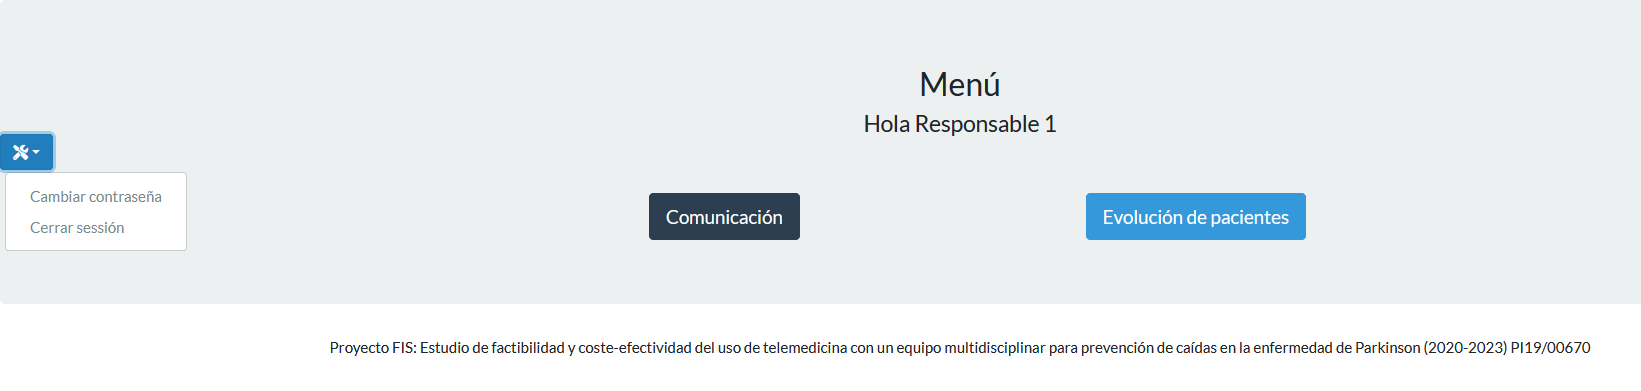
\includegraphics[width=1\textwidth]{menuResponsable}
	\caption{Menú principal de un responsable.}
	\label{fig:menuPaciente}
\end{figure}

\begin{figure}[h]
	\centering
	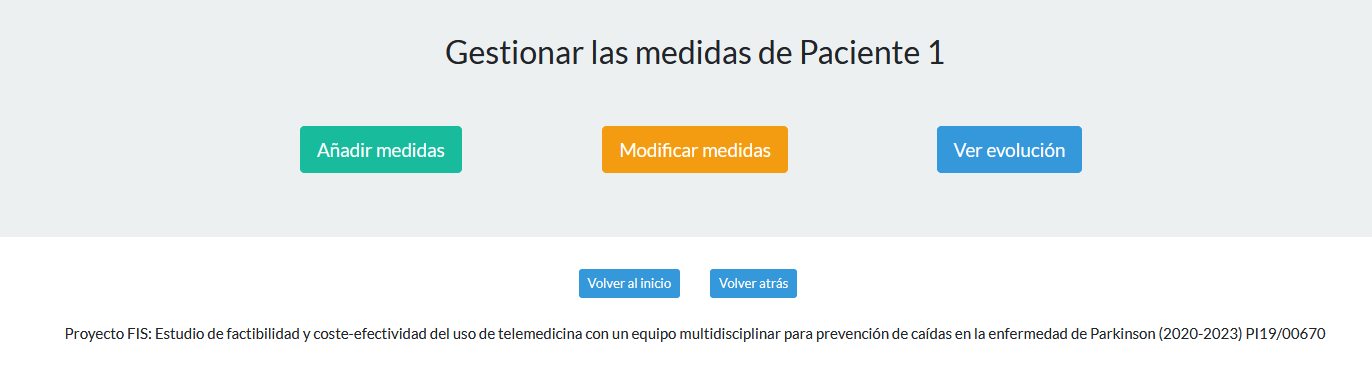
\includegraphics[width=1\textwidth]{menuestad}
	\caption{Menú de estadísticas.}
	\label{fig:menuest}
\end{figure}

\begin{figure}[h]
	\centering
	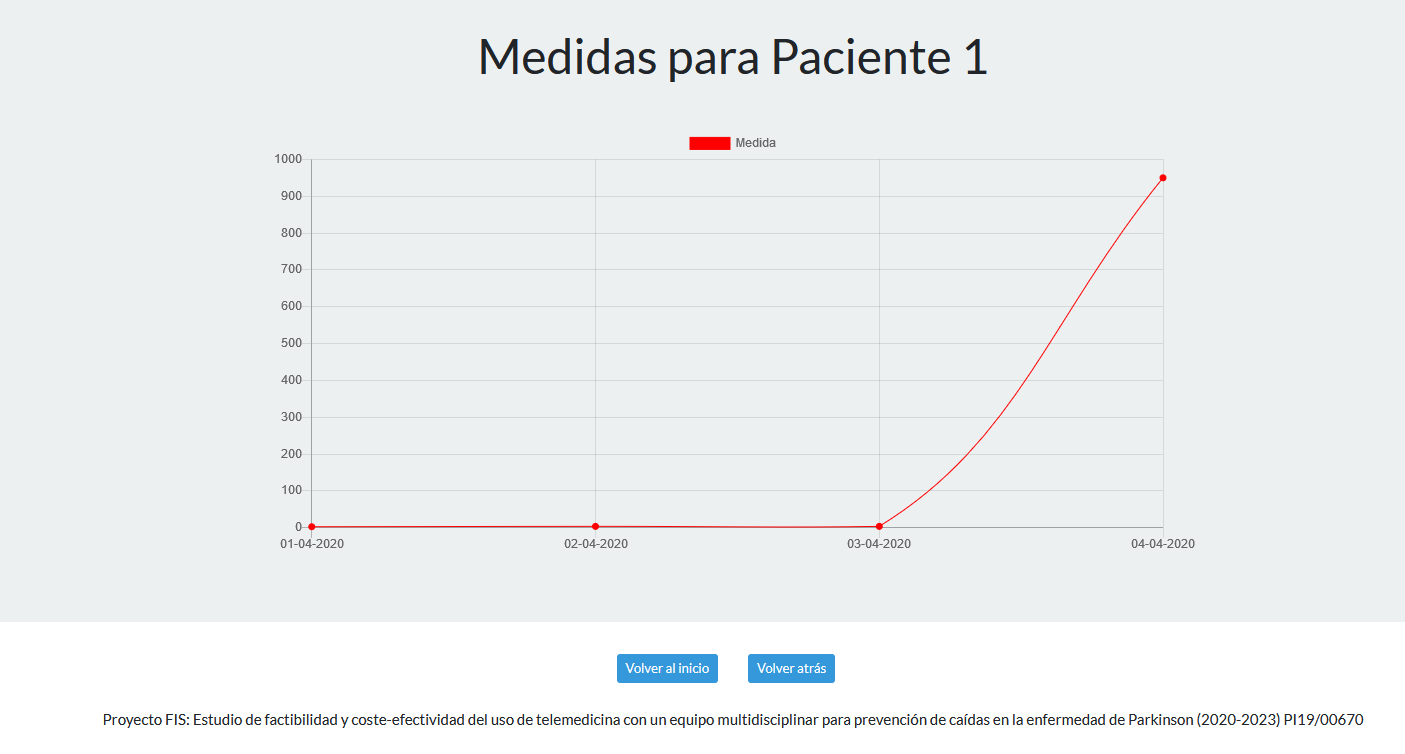
\includegraphics[width=1\textwidth]{ejemploest}
	\caption{Ejemplo de la evolución de un paciente vista por un responsable.}
	\label{fig:ejemploest}
\end{figure}

\subsection{Paciente}
Los pacientes que van a utilizar la aplicación, son pacientesde edad avanzada con Parkinson y riesgo de caídas. Esto se ha tenido muy en cuenta tanto en el diseño como en la creación de la parte de la aplicación orientada en los pacientes, se ha intentado que esta parte sea lo más accesible posible, para que todos los pacientes puedan manejarse bien con la aplicación y así poder sacarle el mayor provecho.

Para poder realizar una aplicación lo más accesible posible primero se ha de saber la forma que van a tener los pacientes de interactuar con ésta. En este caso los pacientes van a utilizar un mando de SNES\footnote{SNES: \textit{Super Nintendo Entertainment System}.} con botones de colores, es por ello que se ha aprovechado estos colores para poder mostrar en la interfaz de la aplicación que botón han de pulsar para realizar que acción. Además, se ha creado un botón de ayuda que carga una página donde se puede ver la acción que realiza cada botón del mando. Un ejemplo de la interfaz de esta aplicación se puede ver en la figura~\ref{fig:menupaciente}.

\begin{figure}[h]
	\centering
	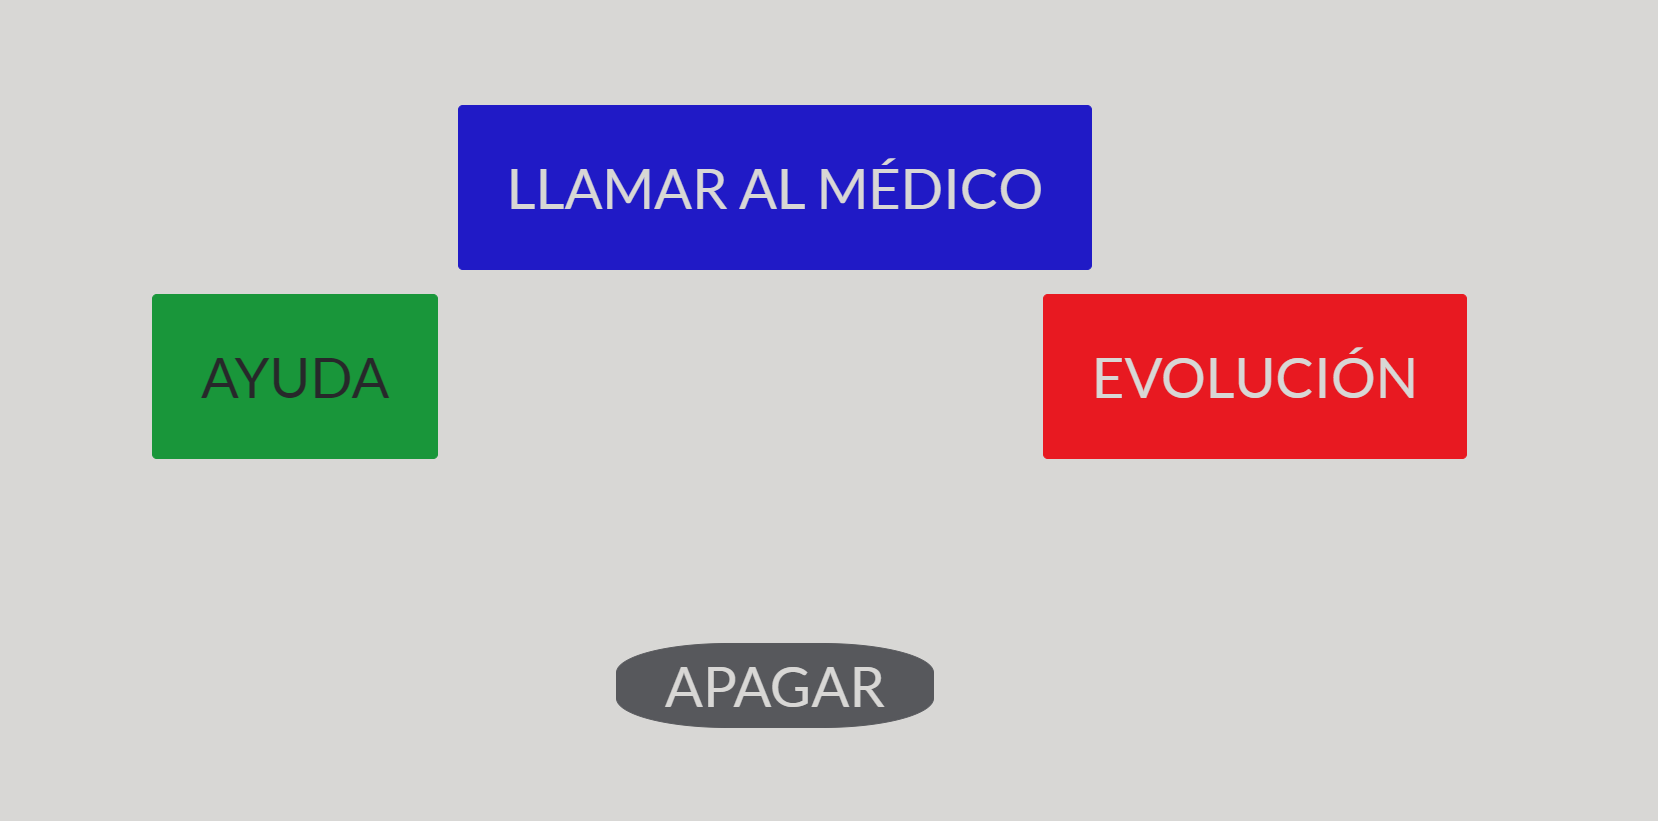
\includegraphics[width=1\textwidth]{menupac}
	\caption{Menú principal de los pacientes.}
	\label{fig:menupaciente}
\end{figure}

\subsection{Dispositivos necesarios}
Para poder utilizar la aplicación se necesitan distintos dispositivos, que dependiendo del tipo de usuario (responsable o paciente) son unos u otros.

Para los responsables lo único que se necesita es un ordenador con conexión a \textit{Internet} y una cámara conectada a éste.

Por otro lado, se presupone que los pacientes no disponen de ningún dispositivo capaz de cargar la aplicación, es por ello que a cada paciente se le proporciona:
\begin{itemize}
	\item Dispositivo: MSI - Cubi N 8GL-001BEU N4000 1,10 GHz Western Digital - Green M.2 120 GB Serial ATA III.
	\item Cámara: Logitech HD Pro WebCam C920.
\end{itemize}

\subsection{Conexión}
Como ya se ha comentado, el principal uso de la aplicación es las rehabilitaciones \textit{online} para pacientes, mayoritariamente de tercera edad, que no se pueden desplazar a las consultas. Muchas de estas personas mayores viven en lugares donde no se tiene contratada ninguna línea de \textit{Internet}, es por ello que además del desarrollo de la aplicación se contrató una serie de \textit{routers} 4G para poder proporcionar conexión a los dispositivos necesarios. 

\section{Investigación algoritmos de visión por computador}
Tras haber desarrollado la versión inicial, donde en un futuro se quiere añadir lo resultados de este proyecto, se pasó a realizar la primera investigación sobre los distintos algoritmos de visión por computar capaces de detectar y seguir los movimientos de una persona. 

De estos algoritmos se necesita:
\begin{itemize}
	\item Posibilidad de cargar un modelo existente o crear un modelo capaz de detectar a la persona que sale en la imagen.
	\item Posibilidad de cargar un modelo existente o crear un modelo capaz de detectar la posición de la persona.
	\item Que el procesado de nuevos fotogramas para detectar a la persona y su posición se realicé en poco tiempo.
	\item Que la salida del procesado de los fotogramas pueda servir para una posterior comparación con el ejercicio base.
\end{itemize}

Teniendo todos estos factores en cuenta se estudió qué herramientas se pueden usar para esta fase del trabajo. Se buscaron herramientas programadas en \textit{Python} para poder conectarse bien con el resto del proyecto y porque es uno de los lenguajes con los cuales se tiene más soltura, tanto por parte del alumno como por parte de los tutores para resolver dudas y ayudar en los problemas. Las herramientas encontradas fuera:
\begin{itemize}
	\item \textit{TF-Pose-Estimator}.
	\item \textit{PoseNet}.
	\item \textit{Detectron2}.
\end{itemize}

De cada una de estas herramientas se realizó una investigación y experimentación para probar si cumplían las necesidades requeridas. Al finalizar esta etapa, la única herramienta que permitía realizar todas las necesidades era \textit{Detectron2}. Además, permite con un modelo ya creado por los propios desarrolladores realizar las tareas de predicción de elementos y de la posición de la persona.

Cabe destacar uno de los grandes problemas que surgió en esta fase, y fue justamente con \textit{Detectron2}, la herramienta elegida. El problema era que las versiones de \textit{CUDA} y de \textit{PyTorch} no eran compatibles. El problema se agrandó al estar trabajando en un \textit{workstation} de la universidad como es \textit{Gamma} que utilizan otros investigadores y también por la compleja estructura del propio computador. Tras hablar con el administrador de la computadora, que es uno de los tutores de este trabajo, el doctor Álvar Arnaiz González, se pudo arreglar el problema actualizando la versión de los \textit{drivers} de \textit{CUDA}, y una vez actualizados descargando la versión compatible de \textit{PyTorch}. 
\section{Investigación de \textit{Detectron2}}
La fase de investigación de \textit{Detectron2} fue una de las más importantes, y por ende, más costosas en tiempo. Fue en esta fase donde se investigaron las distintas formas que tiene la herramienta para crear o importar modelos con los que poder trabajar. Una vez se seleccionó el modelo se realizó otro estudio para ver qué configuración era la más correcta en el problema tratado.

Al ser una de las fases en las que más tiempo se ha dedicado, también es una de las fases donde surgieron más problemas tanto en la creación de los modelos, como en la visualización y el almacenamiento de los resultados obtenidos. Todos estos problemas serán comentados en este apartado.  
\subsection{Selección del modelo}
Tras haber elegido a \textit{Detrectron2} como herramienta de visión por computador para detectar a los pacientes y obtener de estos sus posiciones, elegir qué modelo, dentro de las posibilidades de la herramienta, utilizar para realizar estás tareas.

\textit{Dectectron2} permite dos formas de obtener un modelo:
\begin{itemize}
	\item Crear un modelo propio a partir de una gran cantidad de datos.
	\item Importación de modelos ya entrenados.
\end{itemize}

Ante la falta de datos para la creación de un modelo que diese buenos resultados, y al comprobar en la fase anterior que con la importación de modelos existentes se podían obtener buenos resultados, la investigación se centró en los modelos ya existentes entrenados por los creadores de la herramienta. Estos modelos de redes neuronales fueron entrenados en servidores \textit{Big Basin} de \textit{Facebook}, sucesores de los servidores \textit{Big Sur}, ambos orientados al uso de arquitecturas con varias GPUs potentes para el entrenamiento y uso de algoritmos de inteligencia artificial~\cite{bigbasin}. En concreto, estos modelos fueron entrenados con 8 Nvidia Tesla V100 con \textit{NVLink}, un tecnología que mejorar las interconexiones entre GPUs proporcionando mayor ancho de banda, haciendo el sistema más escalable~\cite{nvlink}. La mejora con otras generaciones de comunicación \textit{inter-GPU} se puede ver en la figura~\ref{fig:nvlink}.

\begin{figure}[h]
	\centering
	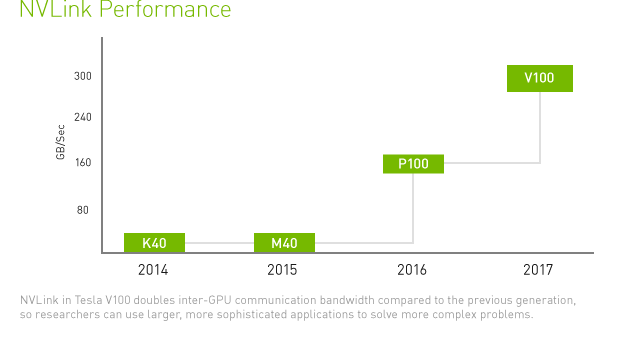
\includegraphics[width=1\textwidth]{nvlink}
	\caption{Mejora del rendimiento en GB/s con NVlink~\cite{nvlink}.}
	\label{fig:nvlink}
\end{figure}

Los modelos creados en \textit{Detectron2} se diferencian en los siguientes tipos:
\begin{itemize}
	\item COCO Detection with Faster R-CNN (Figura~\ref{fig:faster_rcnn_R_50_C4_1x}): modelo que predice los objetos y personas de la imagen.
	\begin{figure}[h]
		\centering
		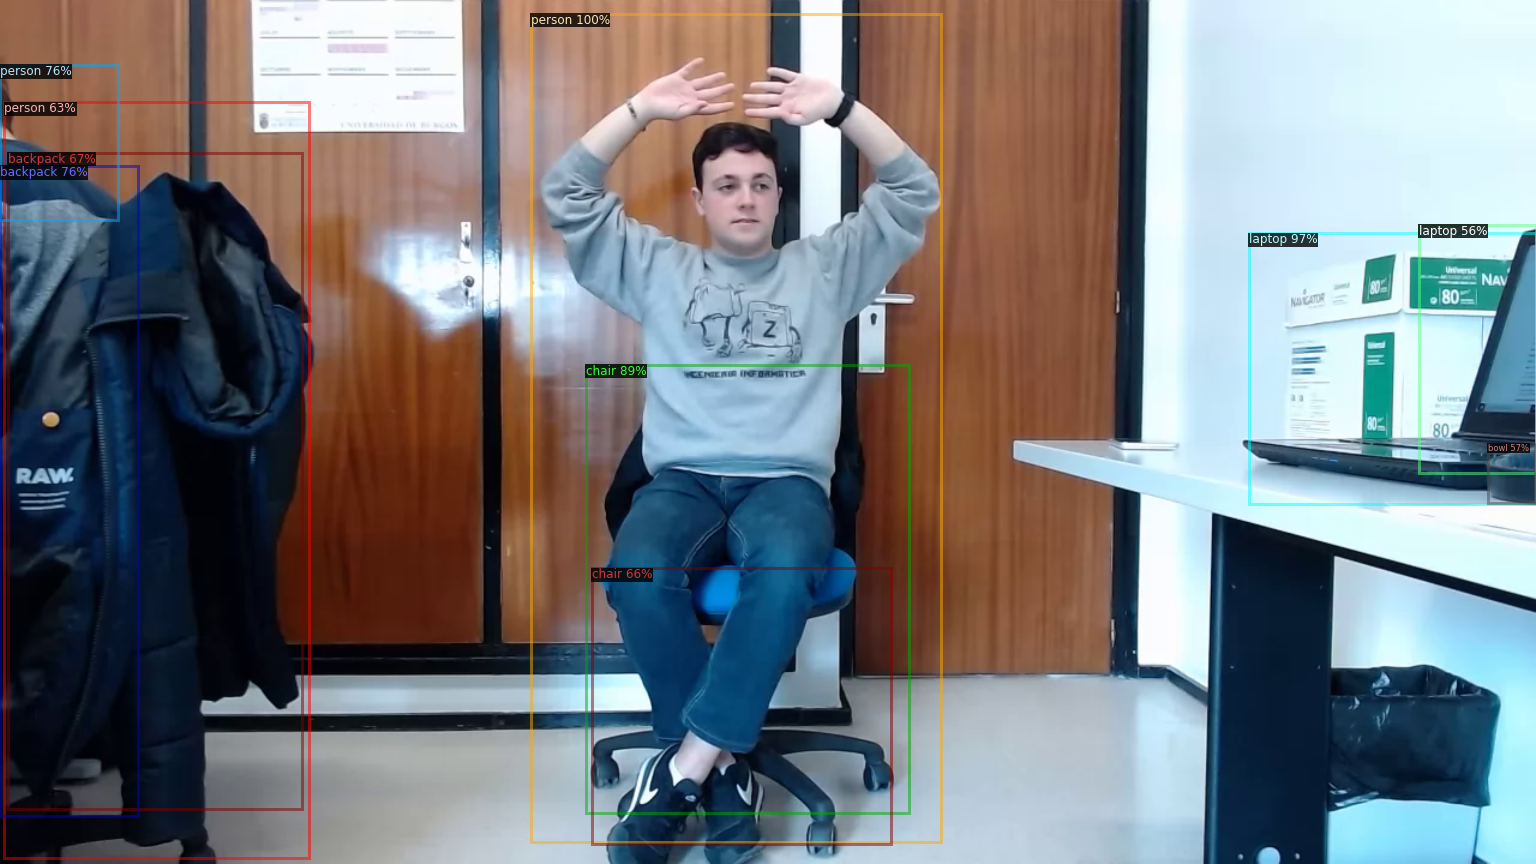
\includegraphics[width=1\textwidth]{faster_rcnn_R_50_C4_1x}
		\caption{Modelo de tipo COCO Detection with Faster R-CNN, \texttt{faster\_rcnn\_R\_50\_C4\_1x}.}
		\label{fig:faster_rcnn_R_50_C4_1x}
	\end{figure}
	\item COCO Detection with RetinaNet (Figura~\ref{fig:retinanet_R_101_FPN_3x}): modelo que detecta objetos y personas. Como se puede ver en la imagen de ejemplo la interpretación no es buena aun utilizando un \textit{threshold} alto.
	\begin{figure}[h]
		\centering
		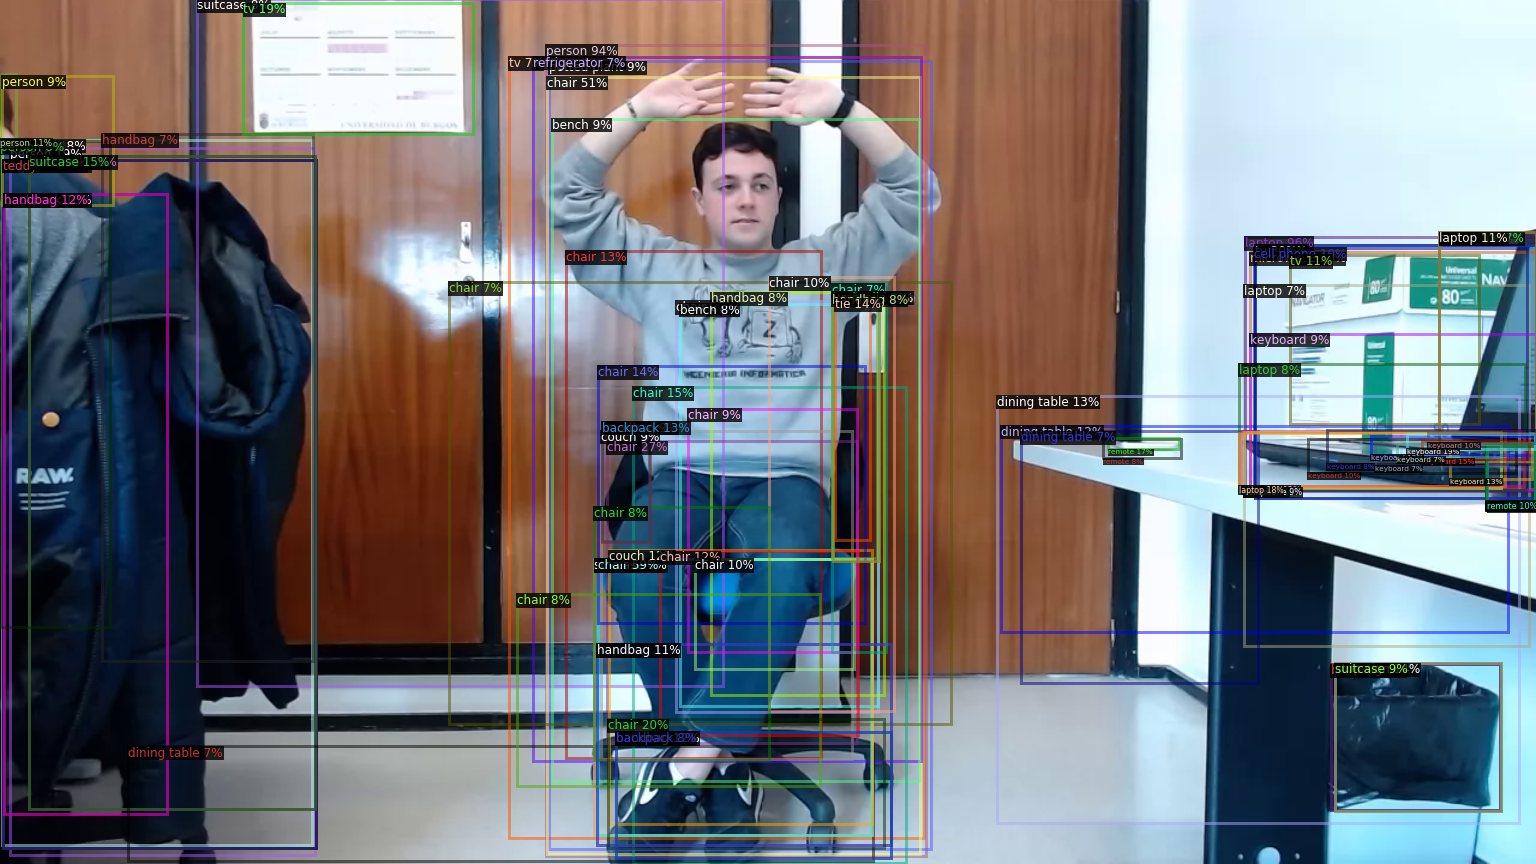
\includegraphics[width=1\textwidth]{retinanet_R_101_FPN_3x}
		\caption{Modelo de tipo COCO Detection with RetinaNet, \texttt{retinanet\_R\_101\_FPN\_3x}.}
		\label{fig:retinanet_R_101_FPN_3x}
	\end{figure}
	\item COCO Detection with RPN and Fast R-CNN: modelos que no se han conseguido probar ya que no siguen la misma estructura que el resto de modelos.
	\item COCO Instance Segmentation Baselines with Mask R-CNN (Figura~\ref{fig:mask_rcnn_R_50_DC5_3x}): modelos de detección de objetos y persona, con delimitación en el área ocupada.
	\begin{figure}[h]
		\centering
		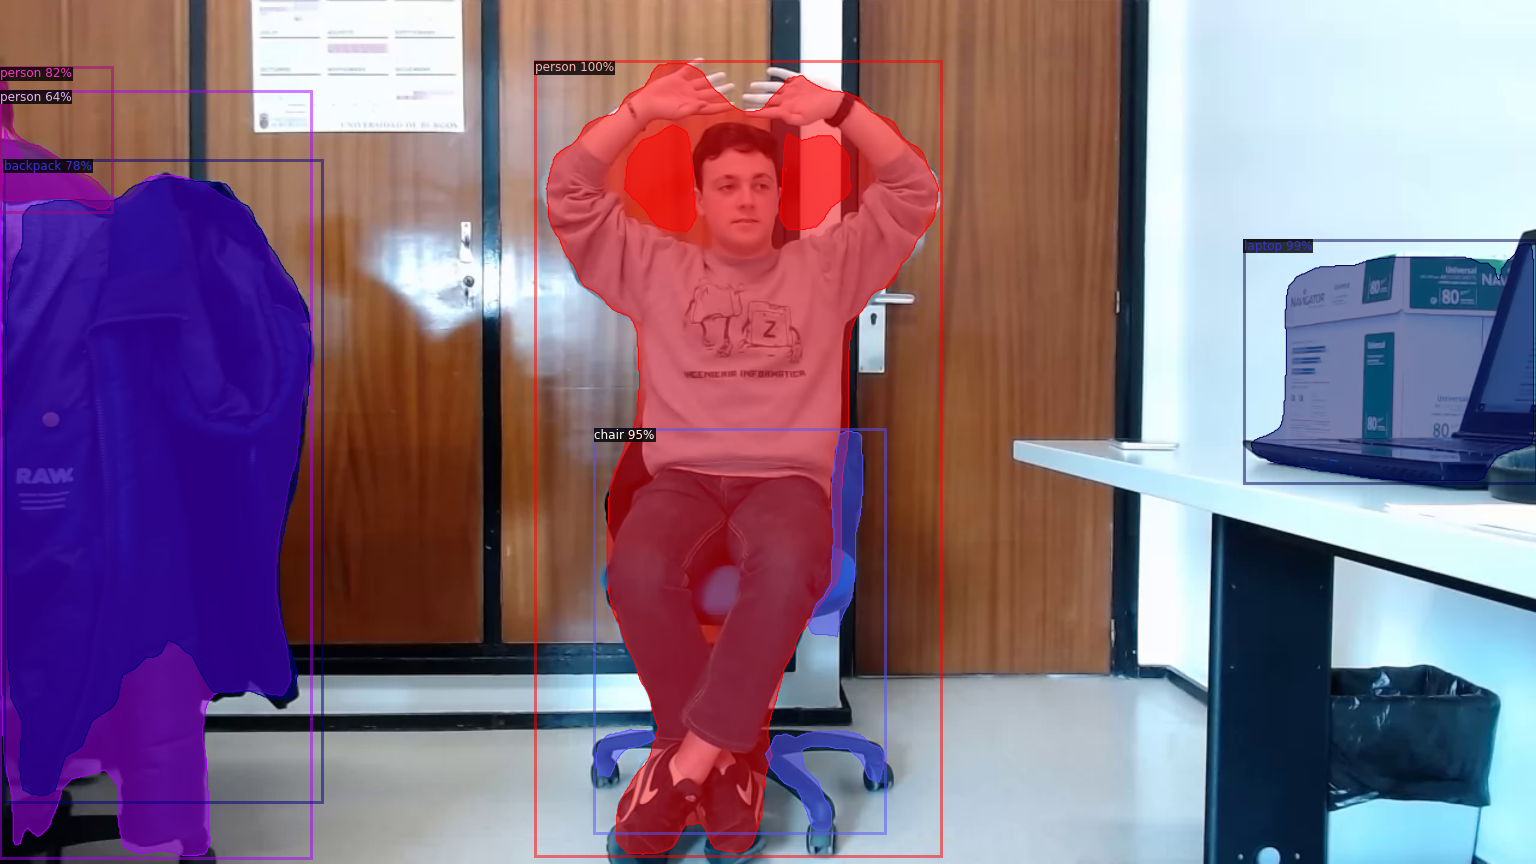
\includegraphics[width=1\textwidth]{mask_rcnn_R_50_DC5_3x}
		\caption{Modelo de tipo COCO Instance Segmentation Baselines with Mask R-CNN, \texttt{mask\_rcnn\_R\_50\_DC5\_3x}.}
		\label{fig:mask_rcnn_R_50_DC5_3x}
	\end{figure}
	\item COCO Person Keypoint Detection Baselines with Keypoint R-CNN (Figura~\ref{fig:keypoint_rcnn_R_101_FPN_3x}): modelos que detectan a las posiciones y unos puntos claves de ellas, estos puntos son nariz, ojos, orejas, hombros, codos, muñecas, cadera, rodilla y tobillos. Como se puede ver en la imagen de ejemplo, estos modelos predicen bastante bien la posición pero a veces detectan otras cosas como personas, por lo que se posteriormente se vio necesario un estudio sobre el \textit{threshold}.
	\begin{figure}[h]
		\centering
		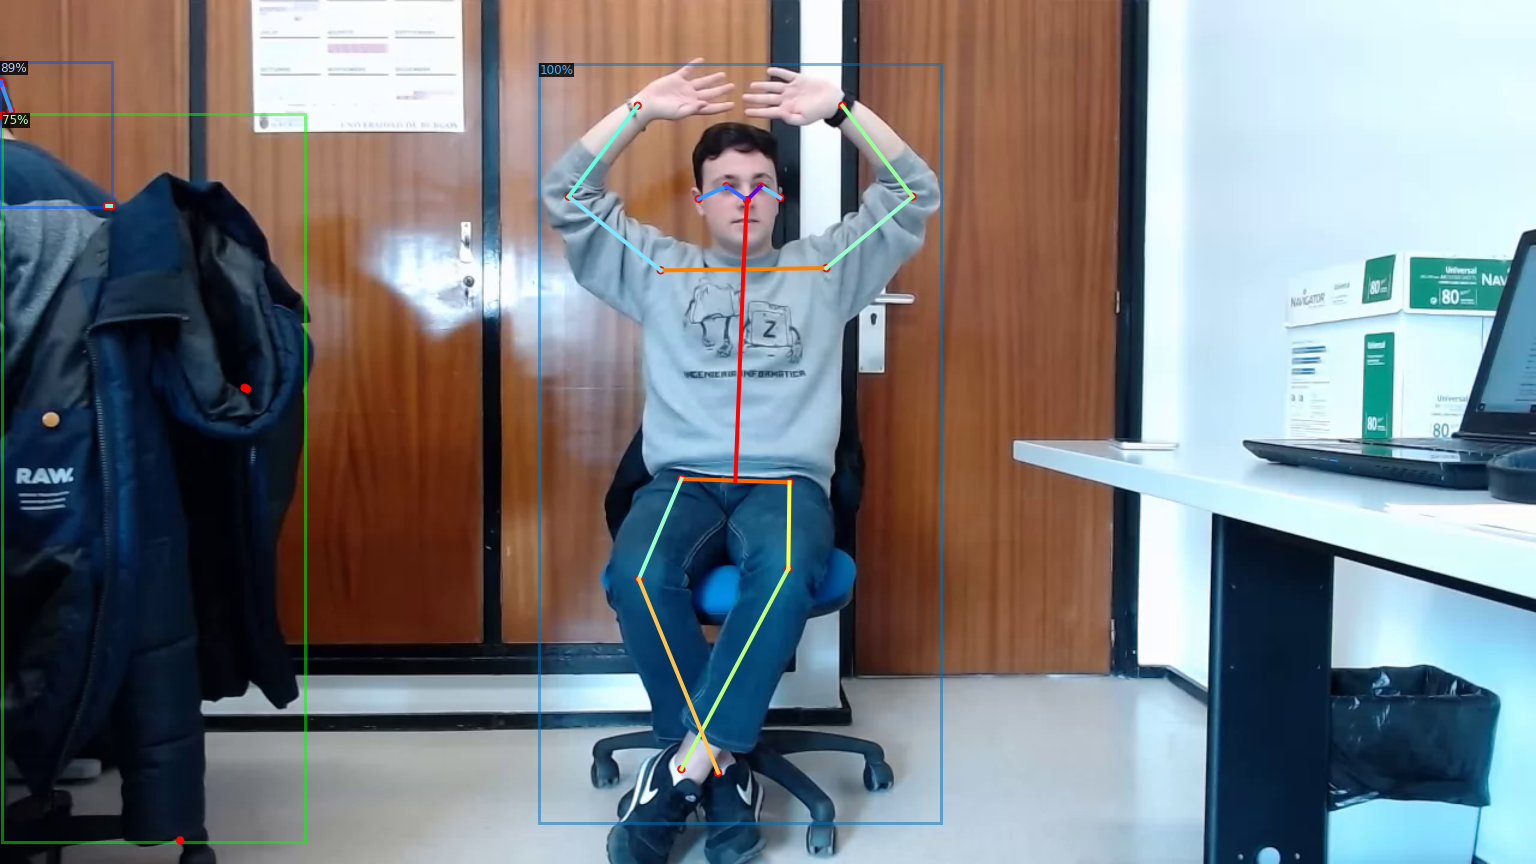
\includegraphics[width=1\textwidth]{keypoint_rcnn_R_101_FPN_3x}
		\caption{Modelo de tipo COCO Person Keypoint Detection Baselines with Keypoint R-CNN, \texttt{keypoint\_rcnn\_R\_101\_FPN\_3x}.}
		\label{fig:keypoint_rcnn_R_101_FPN_3x}
	\end{figure}
	\item COCO Panoptic Segmentation Baselines with Panoptic FPN (Figura~\ref{fig:panoptic_fpn_R_101_3x}): modelos que segmentación como COCO Instance Segmentation Baselines with Mask R-CNN, obtienen resultados muy parecidos.
	\begin{figure}[h]
		\centering
		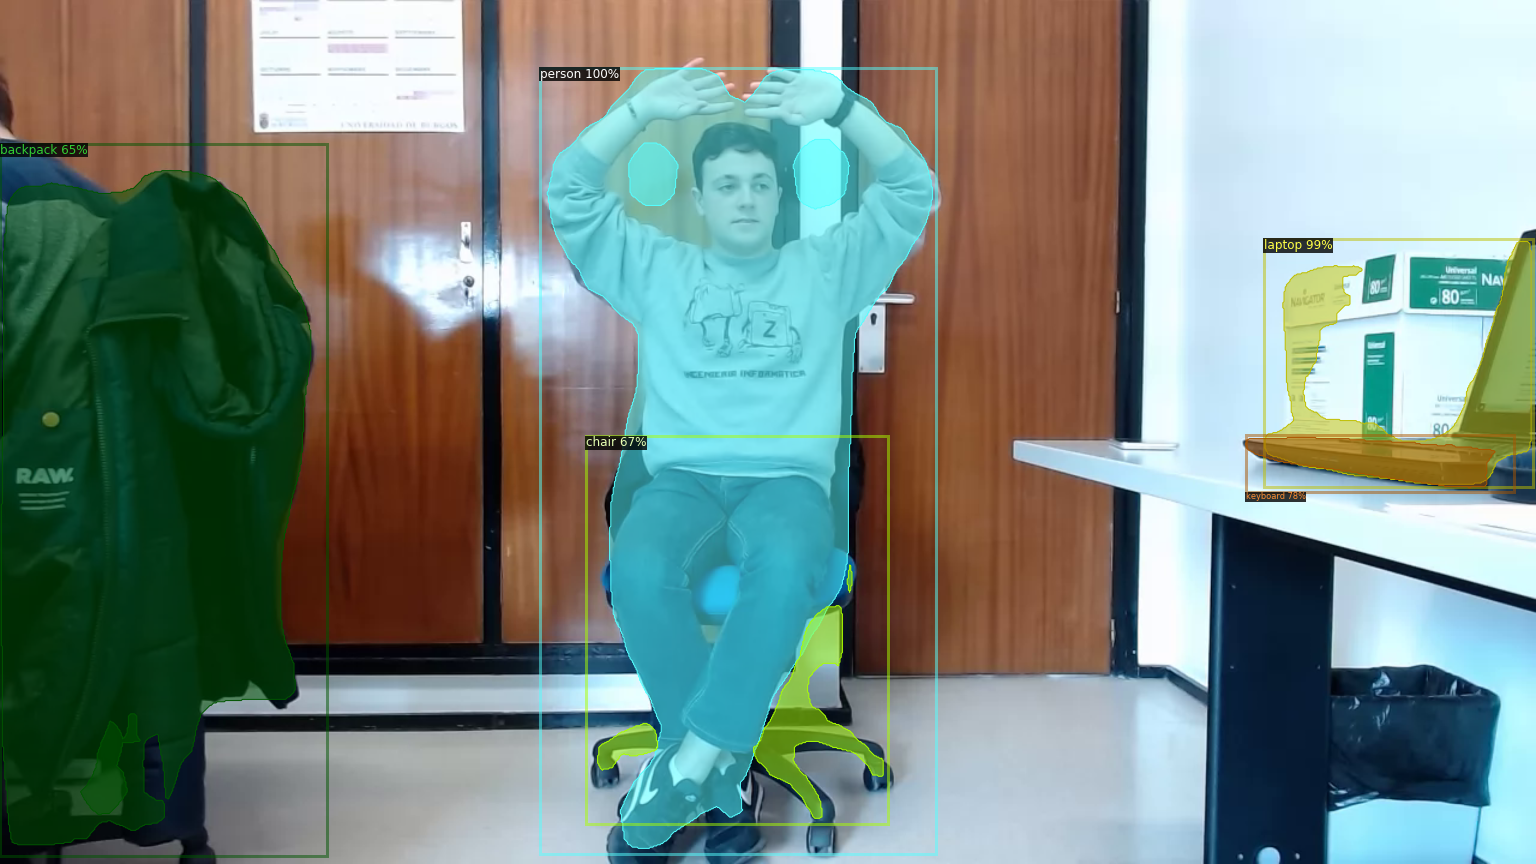
\includegraphics[width=1\textwidth]{panoptic_fpn_R_101_3x}
		\caption{Modelo de tipo COCO Panoptic Segmentation Baselines with Panoptic FPN, \texttt{panoptic\_fpn\_R\_101\_3x}.}
		\label{fig:panoptic_fpn_R_101_3x}
	\end{figure}
	\item LVIS Instance Segmentation Baselines with Mask R-CNN (Figura~\ref{fig:mask_rcnn_X_101_32x8d_FPN_1x}): modelos orientados a la detección de objetos, necesitan un \textit{threshold} bajo para detectar diversos objetos.
	\begin{figure}[h]
		\centering
		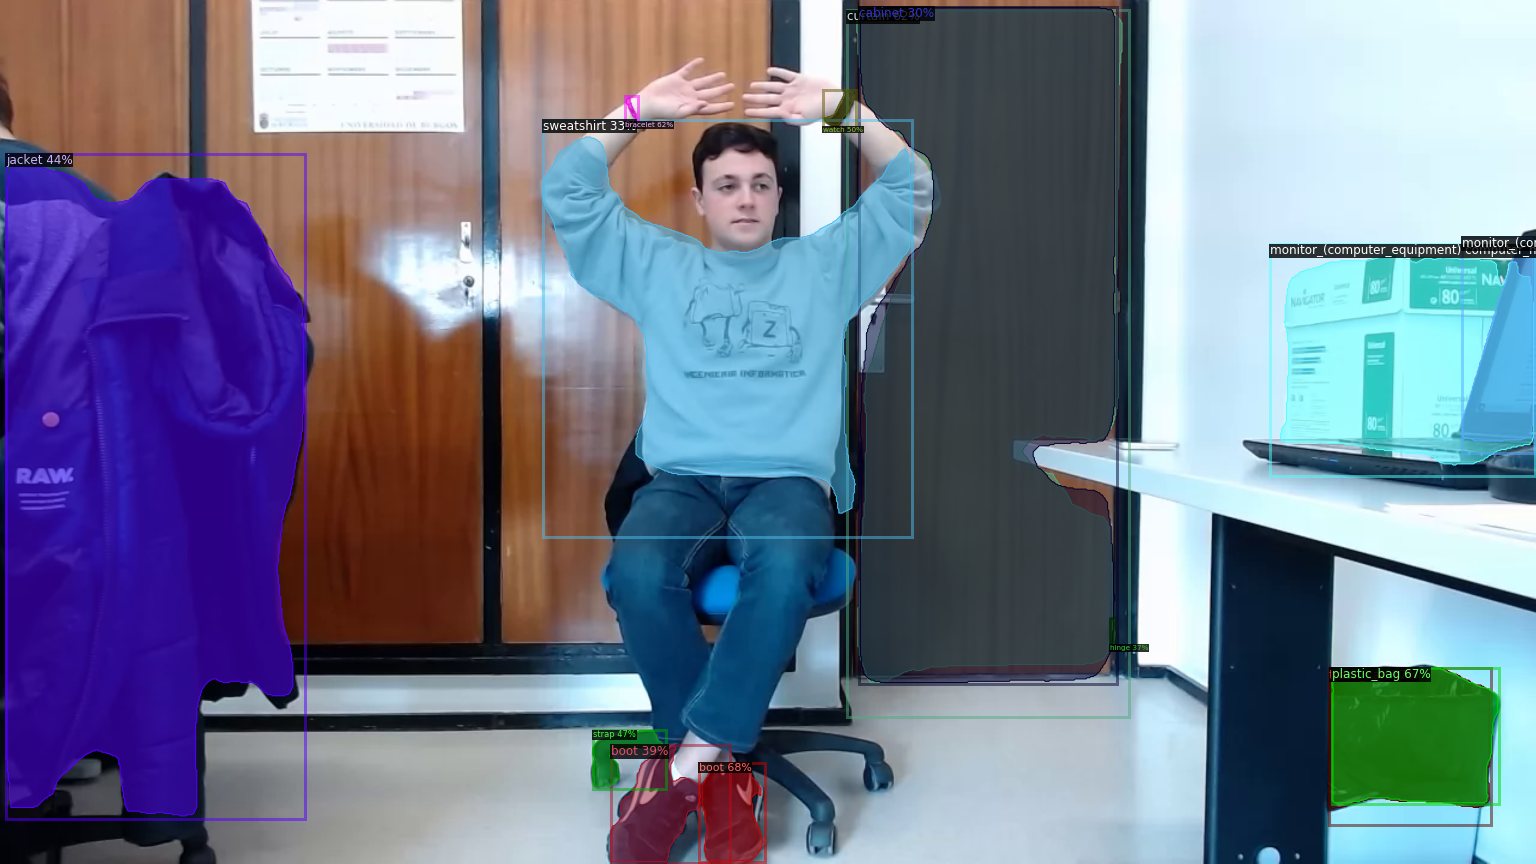
\includegraphics[width=1\textwidth]{mask_rcnn_X_101_32x8d_FPN_1x}
		\caption{Modelo de tipo LVIS Instance Segmentation Baselines with Mask R-CNN, \texttt{mask\_rcnn\_X\_101\_32x8d\_FPN\_1x}.}
		\label{fig:mask_rcnn_X_101_32x8d_FPN_1x}
	\end{figure}
	\item Por último se encuentran modelos como Cityscapes \& Pascal VOC Baselines, otras configuraciones y algoritmos de la primera versión de la herramienta \textit{Detectron}. Estos modelos son muy parecidos a los ya mostrados.
\end{itemize}

Con el estudio de todos los modelos existentes en \textit{Detectron2} se ha comprobado como los únicos modelos que sirven para el problema planteado son COCO Person Keypoint Detection Baselines with Keypoint R-CNN. Dentro de este tipo de modelos existen un total de 4 modelos distintos, para la elección del mejor de estos modelos se realizó otro estudio, esta vez comprobando los tiempos de ejecución, ya que todos los modelos de este tipo realizan unas buenas predicciones (principalmente porque el problema es sencillo, al tener a la persona en el centro de la imagen).

Para realizar este estudio se analizó el tiempo de procesado e impresión de varios vídeos con cada uno de los modelos. Para ello se calculó estos valores para los 4 posibles modelos con un total de 7 vídeos. De este estudio se obtuvieron los resultados que se pueden ver en la tabla~\ref{tab:modelos}.

\begin{table}[h]
	\centering
	\resizebox{\columnwidth}{!}{
\begin{tabular}{l | rrrr}
	\toprule
	\textbf{Modelo} &     \textbf{T. Carga (s)} &       \textbf{T. Procesamiento (s)} &  \textbf{N. Fotogramas} &     \textbf{Periodo} \\
	\midrule
	\texttt{keypoint\_rcnn\_R\_50\_FPN\_3x}     &   9.783479 &  236.774504 &     1989 &  0.119042 \\
	\texttt{keypoint\_rcnn\_R\_50\_FPN\_1x}      &   8.562254 &  237.289880 &     1989 &  0.119301 \\
	\texttt{keypoint\_rcnn\_R\_101\_FPN\_3x}     &  13.017239 &  279.327051 &     1989 &  0.140436 \\
	\texttt{keypoint\_rcnn\_X\_101\_32x8d\_FPN\_3x} &  18.106832 &  422.024270 &     1989 &  0.212179 \\
	\bottomrule
\end{tabular}
}
\caption{Tabla con el estudio de los modelos de posición ordenado por ratio.}
\label{tab:modelos}
\end{table}

Como se puede observar, los datos obtenidos para los modelos son muy parecidos, sobre todo para los dos con menor periodo. Tras observar estos datos se decidió elegir al modelo \texttt{keypoint\_rcnn\_R\_50\_FPN\_3x} (es además el modelo con el que se hicieron las primera pruebas y con el que se decidió a \textit{Detectron2} como herramienta para detectar el movimiento) para utilizarlo en el resto del proyecto. Además, en este estudio se ha podido comprobar que los modelos trabajan correctamente sea cual sea el tipo de ropa que lleve la persona o si pasa un objeto por medio de la imagen (normalmente la posición es correcta, pero como se comentará más adelante a veces algunos fotogramas no son correctos), como se pueden ver en la figuras~\ref{fig:chaqueta} y~\ref{fig:caja}.

Se puede comentar que el modelo seleccionado usa una red neuronal piramidal de tipo FPN con ResNet y RCNN para la detección de la persona, y dentro de la persona sus puntos más importantes.

\begin{figure}[h]
	\centering
	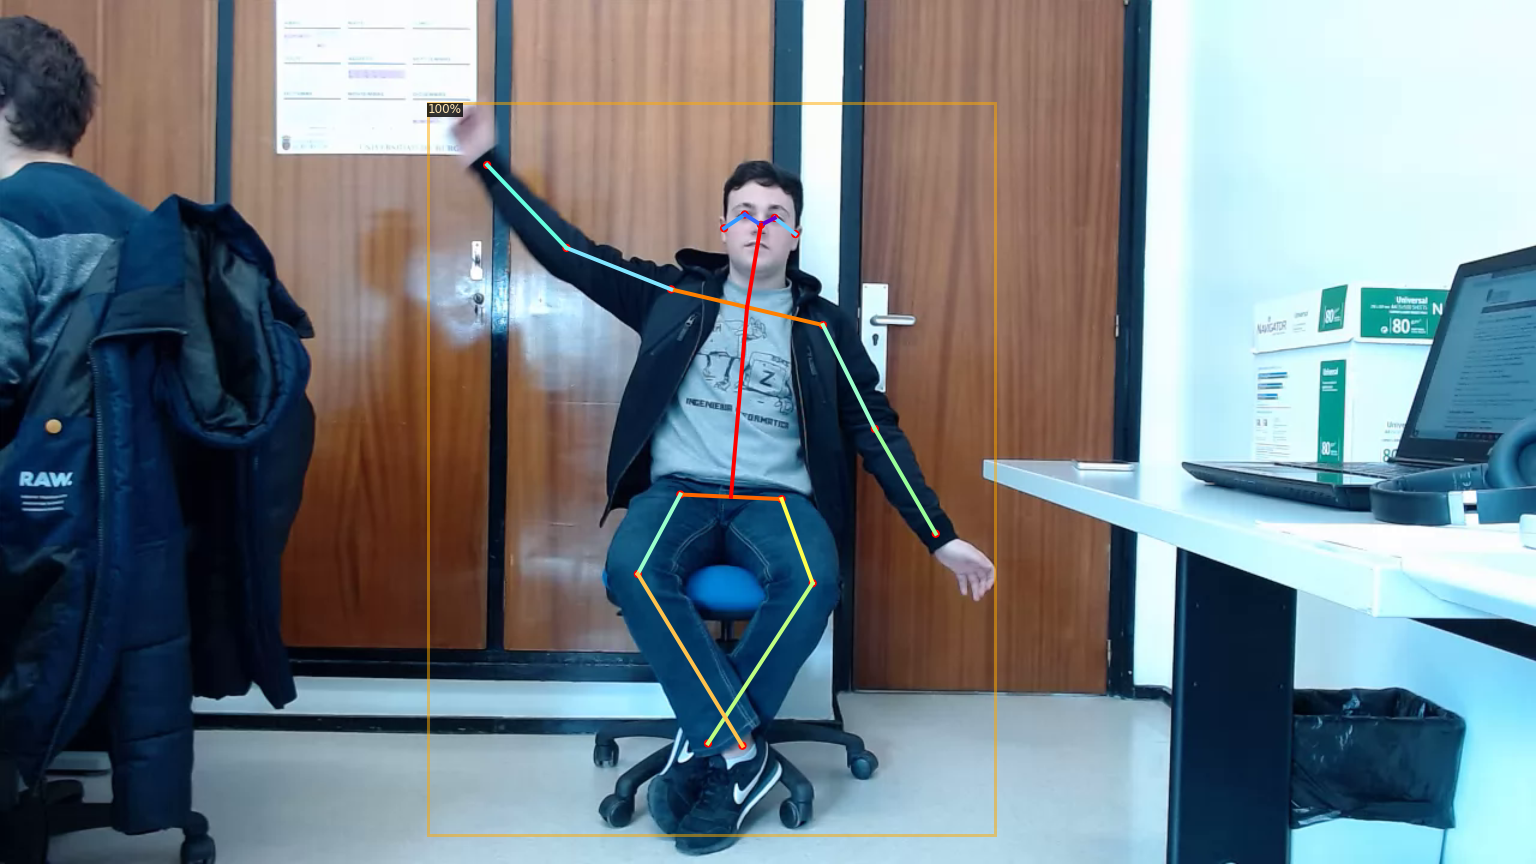
\includegraphics[width=1\textwidth]{chaqueta}
	\caption{Prueba con chaqueta.}
	\label{fig:chaqueta}
\end{figure}

\begin{figure}[h]
	\centering
	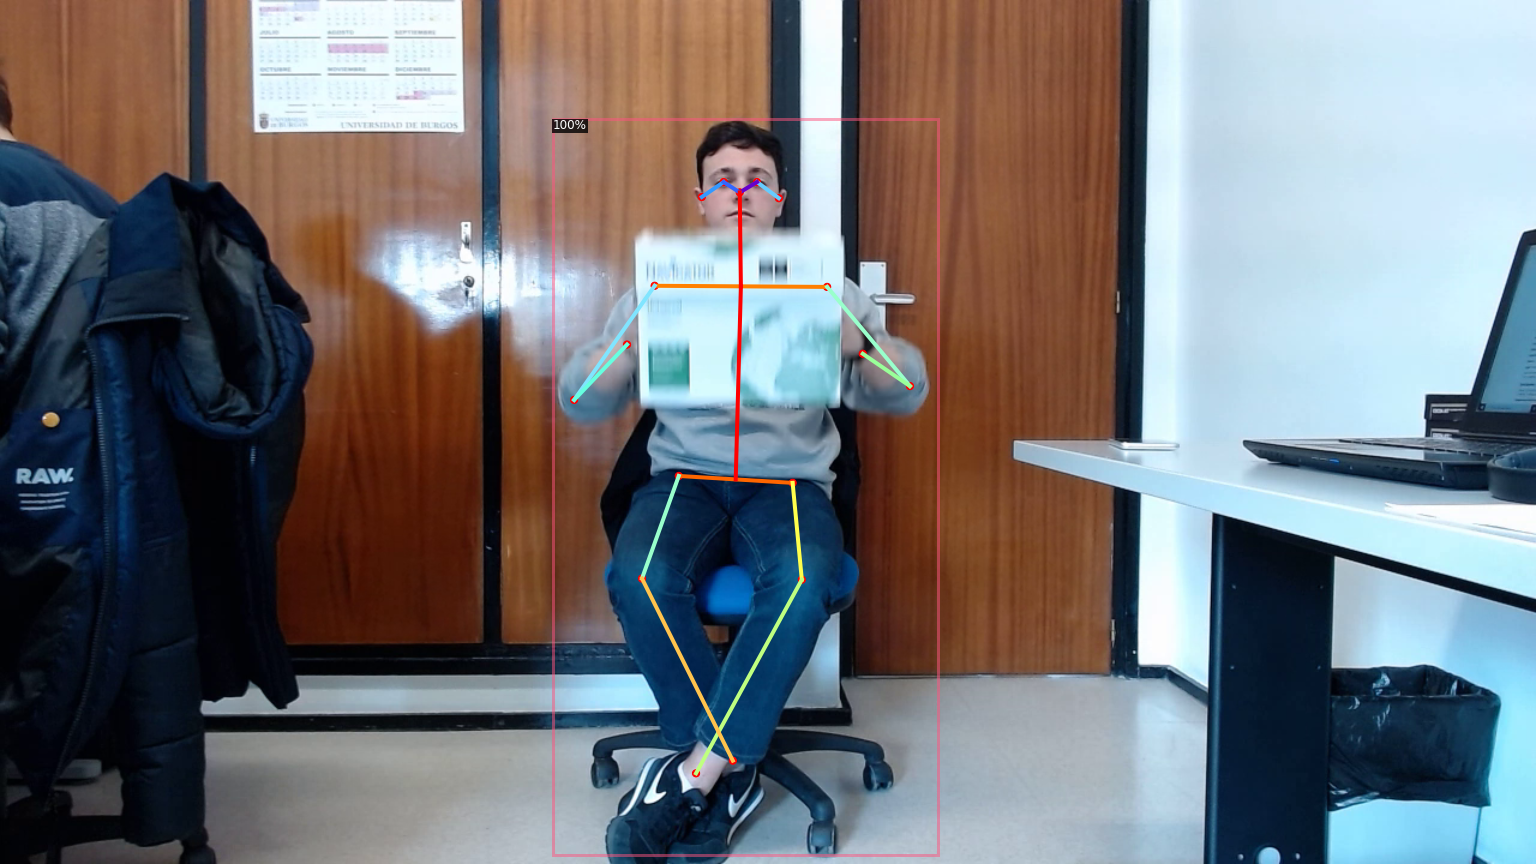
\includegraphics[width=1\textwidth]{caja}
	\caption{Prueba con un objeto de por medio.}
	\label{fig:caja}
\end{figure}


\subsection{Definición del \textit{threshold}}
Como se ha comentado en el apartado anterior, es necesario definir un \textit{threshold}, que es un valor entre 0 y 1 que define la sensibilidad del modelo al detectar, es decir, con valores cercanos a 0 el modelo tiende a detectar más elementos (muchos de ellos erróneos) y cuanto más cercano a 1 menos sensible es, solo detectando los elementos más claros. Sobre este valor se ha realizado un estudio de posibles valores, los valores probados fueron 0.3, 0.5, 0.75 y 0.99.

Con valores bajos del \textit{threshold} se observa que se detectan cosas que no son personas, o se detectan personas que no salen completas en la imagen, como se puede observar en el figura~\ref{fig:pruebaCon0.3}. Esto ocurre con los valores 0.3, 0.5 y 0.75 que dan la misma salida. Sin embargo, con el valor 0.99, como se puede ver en la figura~\ref{fig:pruebaCon0.99}, se obtienen muy buenos resultados detectando únicamente a la persona que aparece en el centro de la imagen, con la posición exacta en todos los puntos.

\begin{figure}[h]
	\centering
	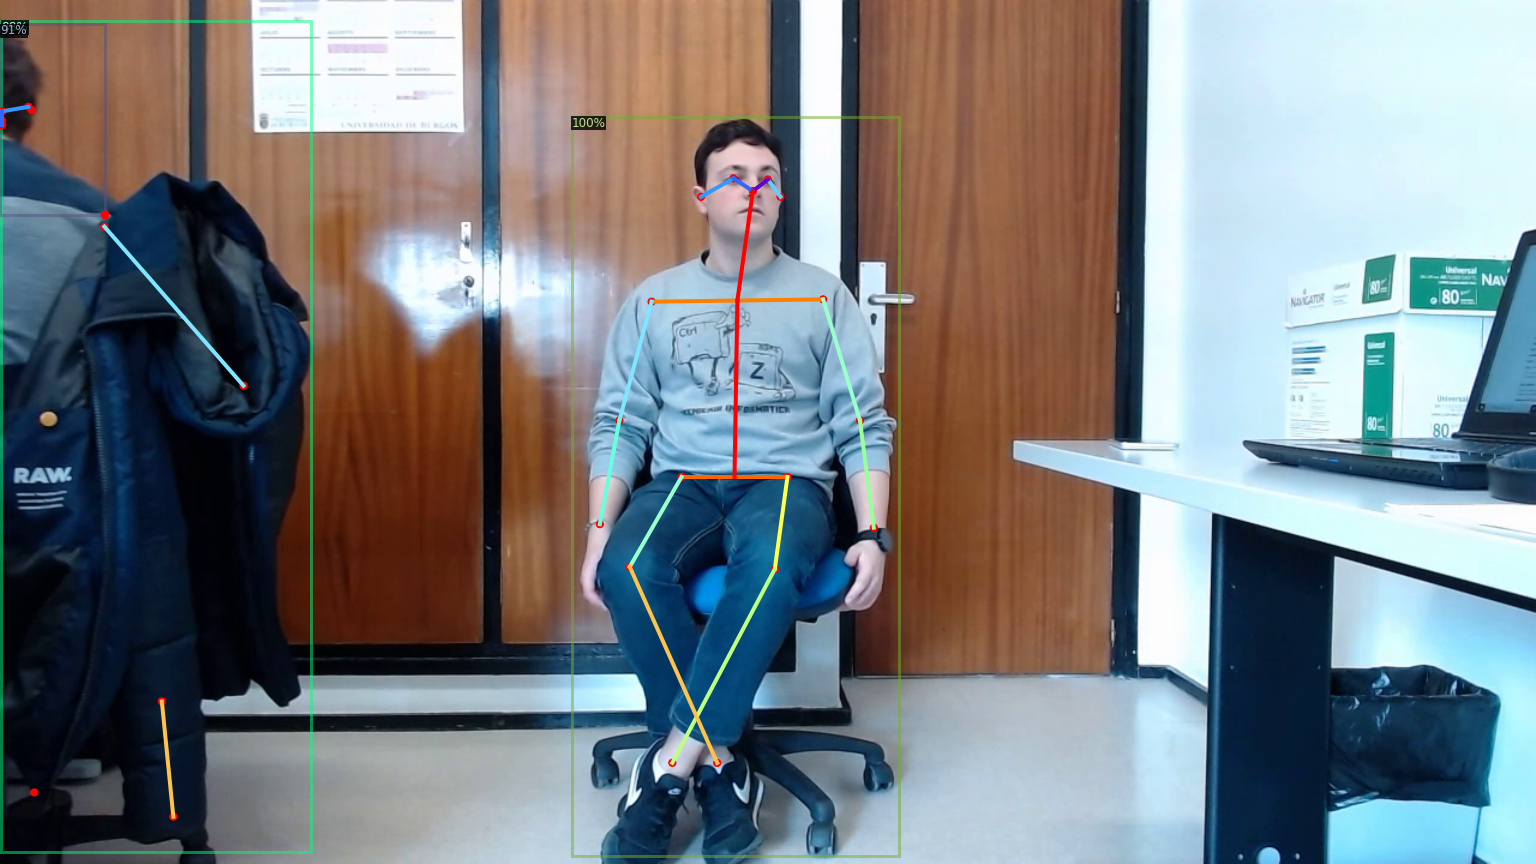
\includegraphics[width=1\textwidth]{pruebaCon0.3}
	\caption{Prueba con \textit{threshold} a 0.3.}
	\label{fig:pruebaCon0.3}
\end{figure}

\begin{figure}[h]
	\centering
	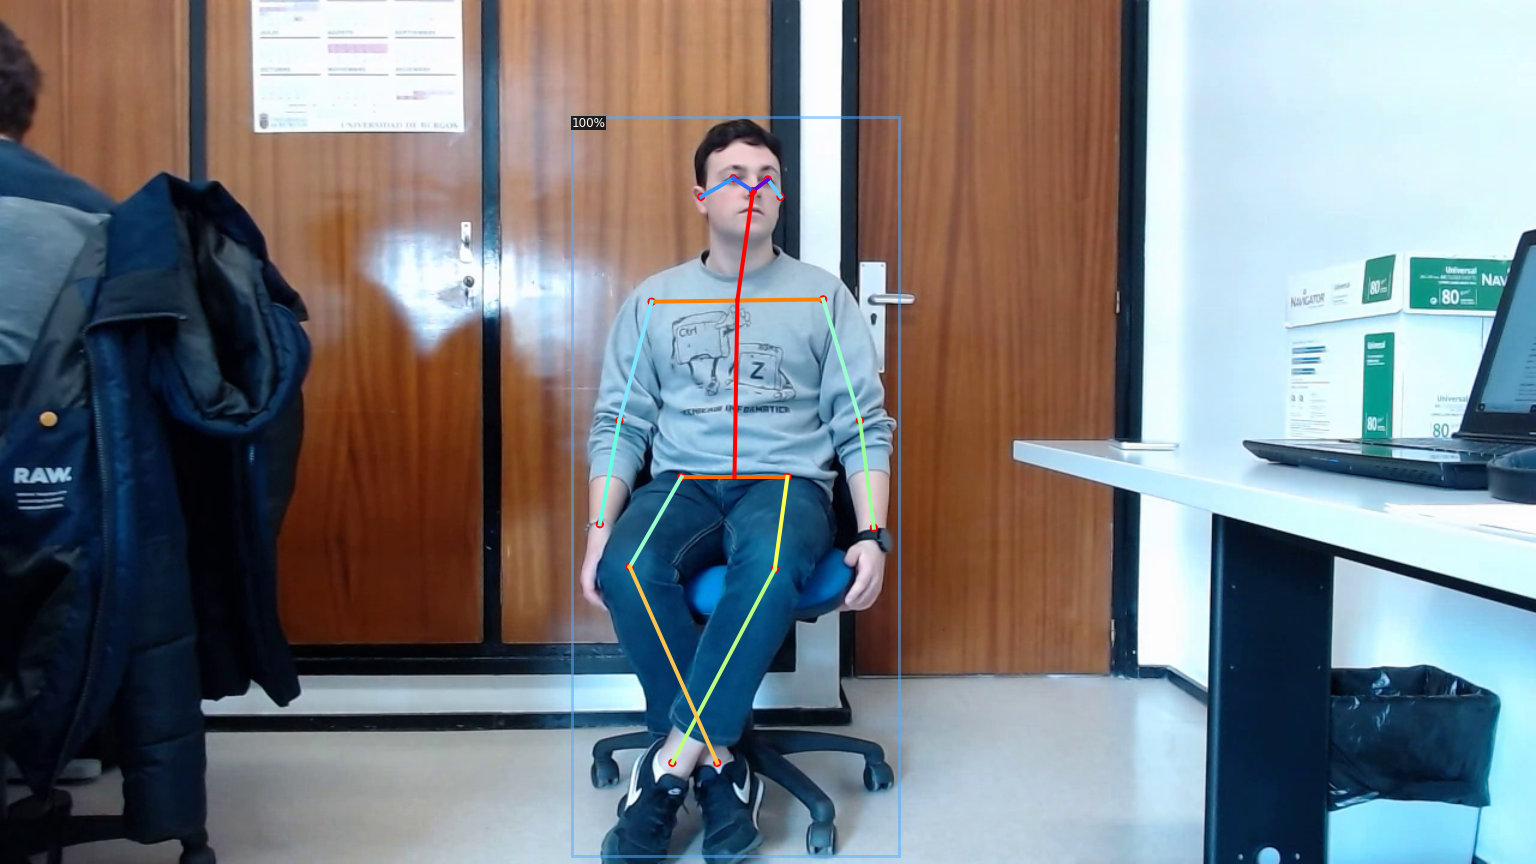
\includegraphics[width=1\textwidth]{pruebaCon0.99}
	\caption{Prueba con \textit{threshold} a 0.99.}
	\label{fig:pruebaCon0.99}
\end{figure}

\subsection{Problemas surgidos}
Como se ha comentado a lo largo del apartado, han surgido distintos problemas que se pueden resumir en:
\begin{itemize}
	\item Problema con los modelos COCO Detection with RPN and Fast R-CNN, que al no tener la misma estructura que el resto de modelos de \textit{Detectron2} no se ha podido probar.
	\item Se intentó almacenar los vídeos procesados pero por problemas con \textit{OpenCV} no se pudo guardar en esta etapa.
\end{itemize}

\section{Cálculo de características}
Una vez se seleccionó el modelo que se iba a utilizar durante todo el proyecto y se determinó el parámetro \textit{threshold} de los modelos, el siguiente paso fue la interpretación de las salidas del modelo. Y después de haber interpretado con el modelo de \textit{Detectron2} una posición ser capaces de calcular características que definan de la mejor manera los datos.
\subsection{Interpretación de las predicciones}
Si se analiza la salida tras predecir un imagen con el predictor creado (DefaultPredictor), se observa que devuelve un diccionario con una única entrada llamada <<instances>> donde se almacena toda la información. Dentro de la instancia existen los siguientes apartados:
\begin{itemize}
	\item \texttt{pred\_boxes}: Boxes, estructura propia de \textit{Dectectron2} donde se almacenan límites de donde entiende que está la persona en un \textit{tensor}, si se ha detectado más de una persona este Boxes estará creado por varios \textit{tensors}.
	\item \texttt{scores}: \textit{tensor} con las probabilidades de que los elementos sean personas. Es este el valor que se compara con el \textit{threshold} para ver si se toma o no como una persona. Si existe más de un valor estos están ordenados de mayor a menor, este es el orden que se sigue en el resto de valores.
	\item \texttt{pred\_classes}: \textit{tensor} con el índice de la clase, en este caso todos los elementos son 0 ya que solo detecta personas, que se identifican con este índice.
	\item \texttt{pred\_keypoints}: \textit{tensor} con todos los puntos clave de cada elemento (persona) detectada. De cada elemento detectado, si la predicción ha sido correcta, se obtienen un total de 17 puntos, con sus valores $x$ e $y$. Después de investigar el posicionamiento de estos puntos se puede decir, como se ve en la figura~\ref{fig:puntos}, que los puntos representan (teniendo en cuenta que se han detectado todos los puntos y que la persona está mirando de frente al objetivo):
	\begin{itemize}
		\item 0: nariz.
		\item 1 y 2: ojo izquierdo y derecho.
		\item 3 y 4: oreja izquierda y derecha.
		\item 5 y 6: hombro izquierdo y derecho.
		\item 7 y 8: codo izquierdo y derecho.
		\item 9 y 10: muñeca izquierda y derecha.
		\item 11 y 12: parte izquierda de la cadera y derecha.
		\item 13 y 14: rodilla izquierda y derecha.
		\item 15 y 16: tobillo izquierdo y derecho.
	\end{itemize}
\end{itemize}

\begin{figure}[h]
	\centering
	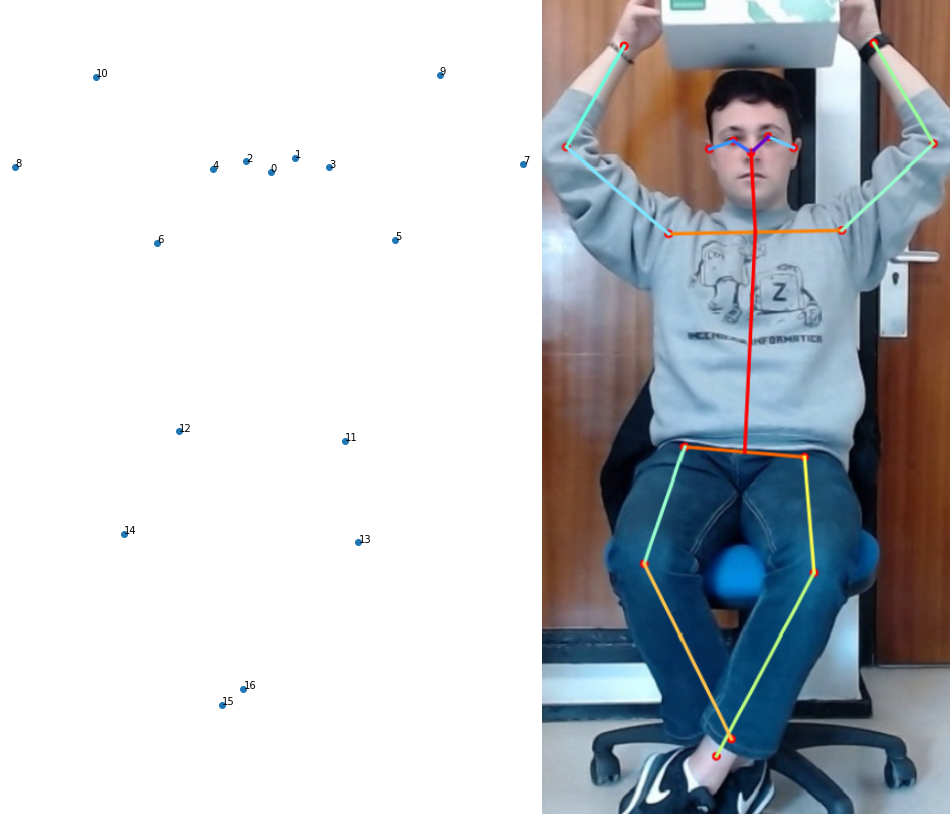
\includegraphics[width=1\textwidth]{puntos}
	\caption{Puntos clave predichos con el modelo junto con la etiqueta con su orden.}
	\label{fig:puntos}
\end{figure}
\subsection{Clase de posición}
Una vez se conoce la salida de las predicciones se puede usar esta para obtener más información de la posición de la persona, que en futuras etapas fue usada para la comparación de posiciones. Por ello se creó una clase que almacena todos los puntos detectados además de realizar cálculos para extraer más características.

Para poder obtener más información sobre los puntos se crearon una serie de funciones que permiten el cálculo de:
\begin{itemize}
	\item Cálculo de puntos medios. Este cálculo se realiza para obtener el punto inferior del cuello que se calcula como el punto medio de la recta que une los dos hombros y se utiliza también para calcular el punto central de la cadera a partir de su punto izquierdo y derecho.
	\item Cálculo de la distancia entre puntos. Este punto se ha realizado sobre todos los pares de puntos unidos. Se pueden utilizar para intuir profundidades.
	\item Cálculo de los ángulos en grados. Este cálculo se ha realizado en todas las combinaciones posibles (conjunto de 3 puntos consecutivos), ya que se cree que son las características que más información van a aportar debido a que no dependen de ningún otro valor como puede ser la profundidad a la que está el paciente, su altura...
\end{itemize}

Como se comentó en apartados anteriores, una vez se tienen los puntos, se ha de realizar una serie de comprobaciones para saber si las posiciones son válidas:
\begin{itemize}
	\item Si existe más de una persona detectada se selecciona la primera, ya que es la que tiene un mayor \textit{score} y por lo tanto el modelo cree que puede ser con mayor probabilidad una persona.
	\item Si una predicción no dispone de todos los puntos no se tiene en cuenta. En la práctica con las pruebas que se han realizado esto solo pasa cuando se pasa un objeto por ciertos puntos del cuerpo, cuando ocurre estos hay algunos fotogramas, muy pocos, que no detectan todos los puntos.
\end{itemize}

\section{Primeras versiones comparación de posiciones} \label{PrimeraVersion}
Una vez se había comprobado que el sistema de cálculo de posiciones era correcto se pasó a la parte final del desarrollo del proyecto, la comparación de posiciones. Para esta primera versión de la comparación de posiciones se decidió usar los ángulos calculados a partir de los puntos y puntos medios de las posiciones. Se decidió usar los ángulos ya que es la única medida calculada que no depende de la posición del usuario grabado.
\subsection{División de la comparación}
La principal característica, a parte del uso de los ángulos, de la primera versión de la comparación de posiciones fue la división de la comparación en distintas partes para poder dar un peso mayor o menor a cada una de ellas. Esto se vio necesario observan los vídeos de ejemplos de los ejercicios que se proporcionaron, ya que había ejercicios donde se centraban en los brazos, otros en las piernas...

La división que se planteó en esta versión es (Figura~\ref{fig:estiradosAbajo2}):
\begin{itemize}
	\item Brazos: en esta parte se encuentran unicamente los ángulos de los codos de ambos brazos (5 y 6).
	\item Torso: ángulos de la cadera con la columna (7 y 8), ángulos de los hombros (3 y 4) y ángulos del cuello con respecto a los hombros (1 y 2).
	\item Piernas: ángulos de la cadera con el fémur de cada pierna (9 y 10) y ángulos de cada rodilla (11 y 12).
\end{itemize}

\begin{figure}[h]
	\centering
	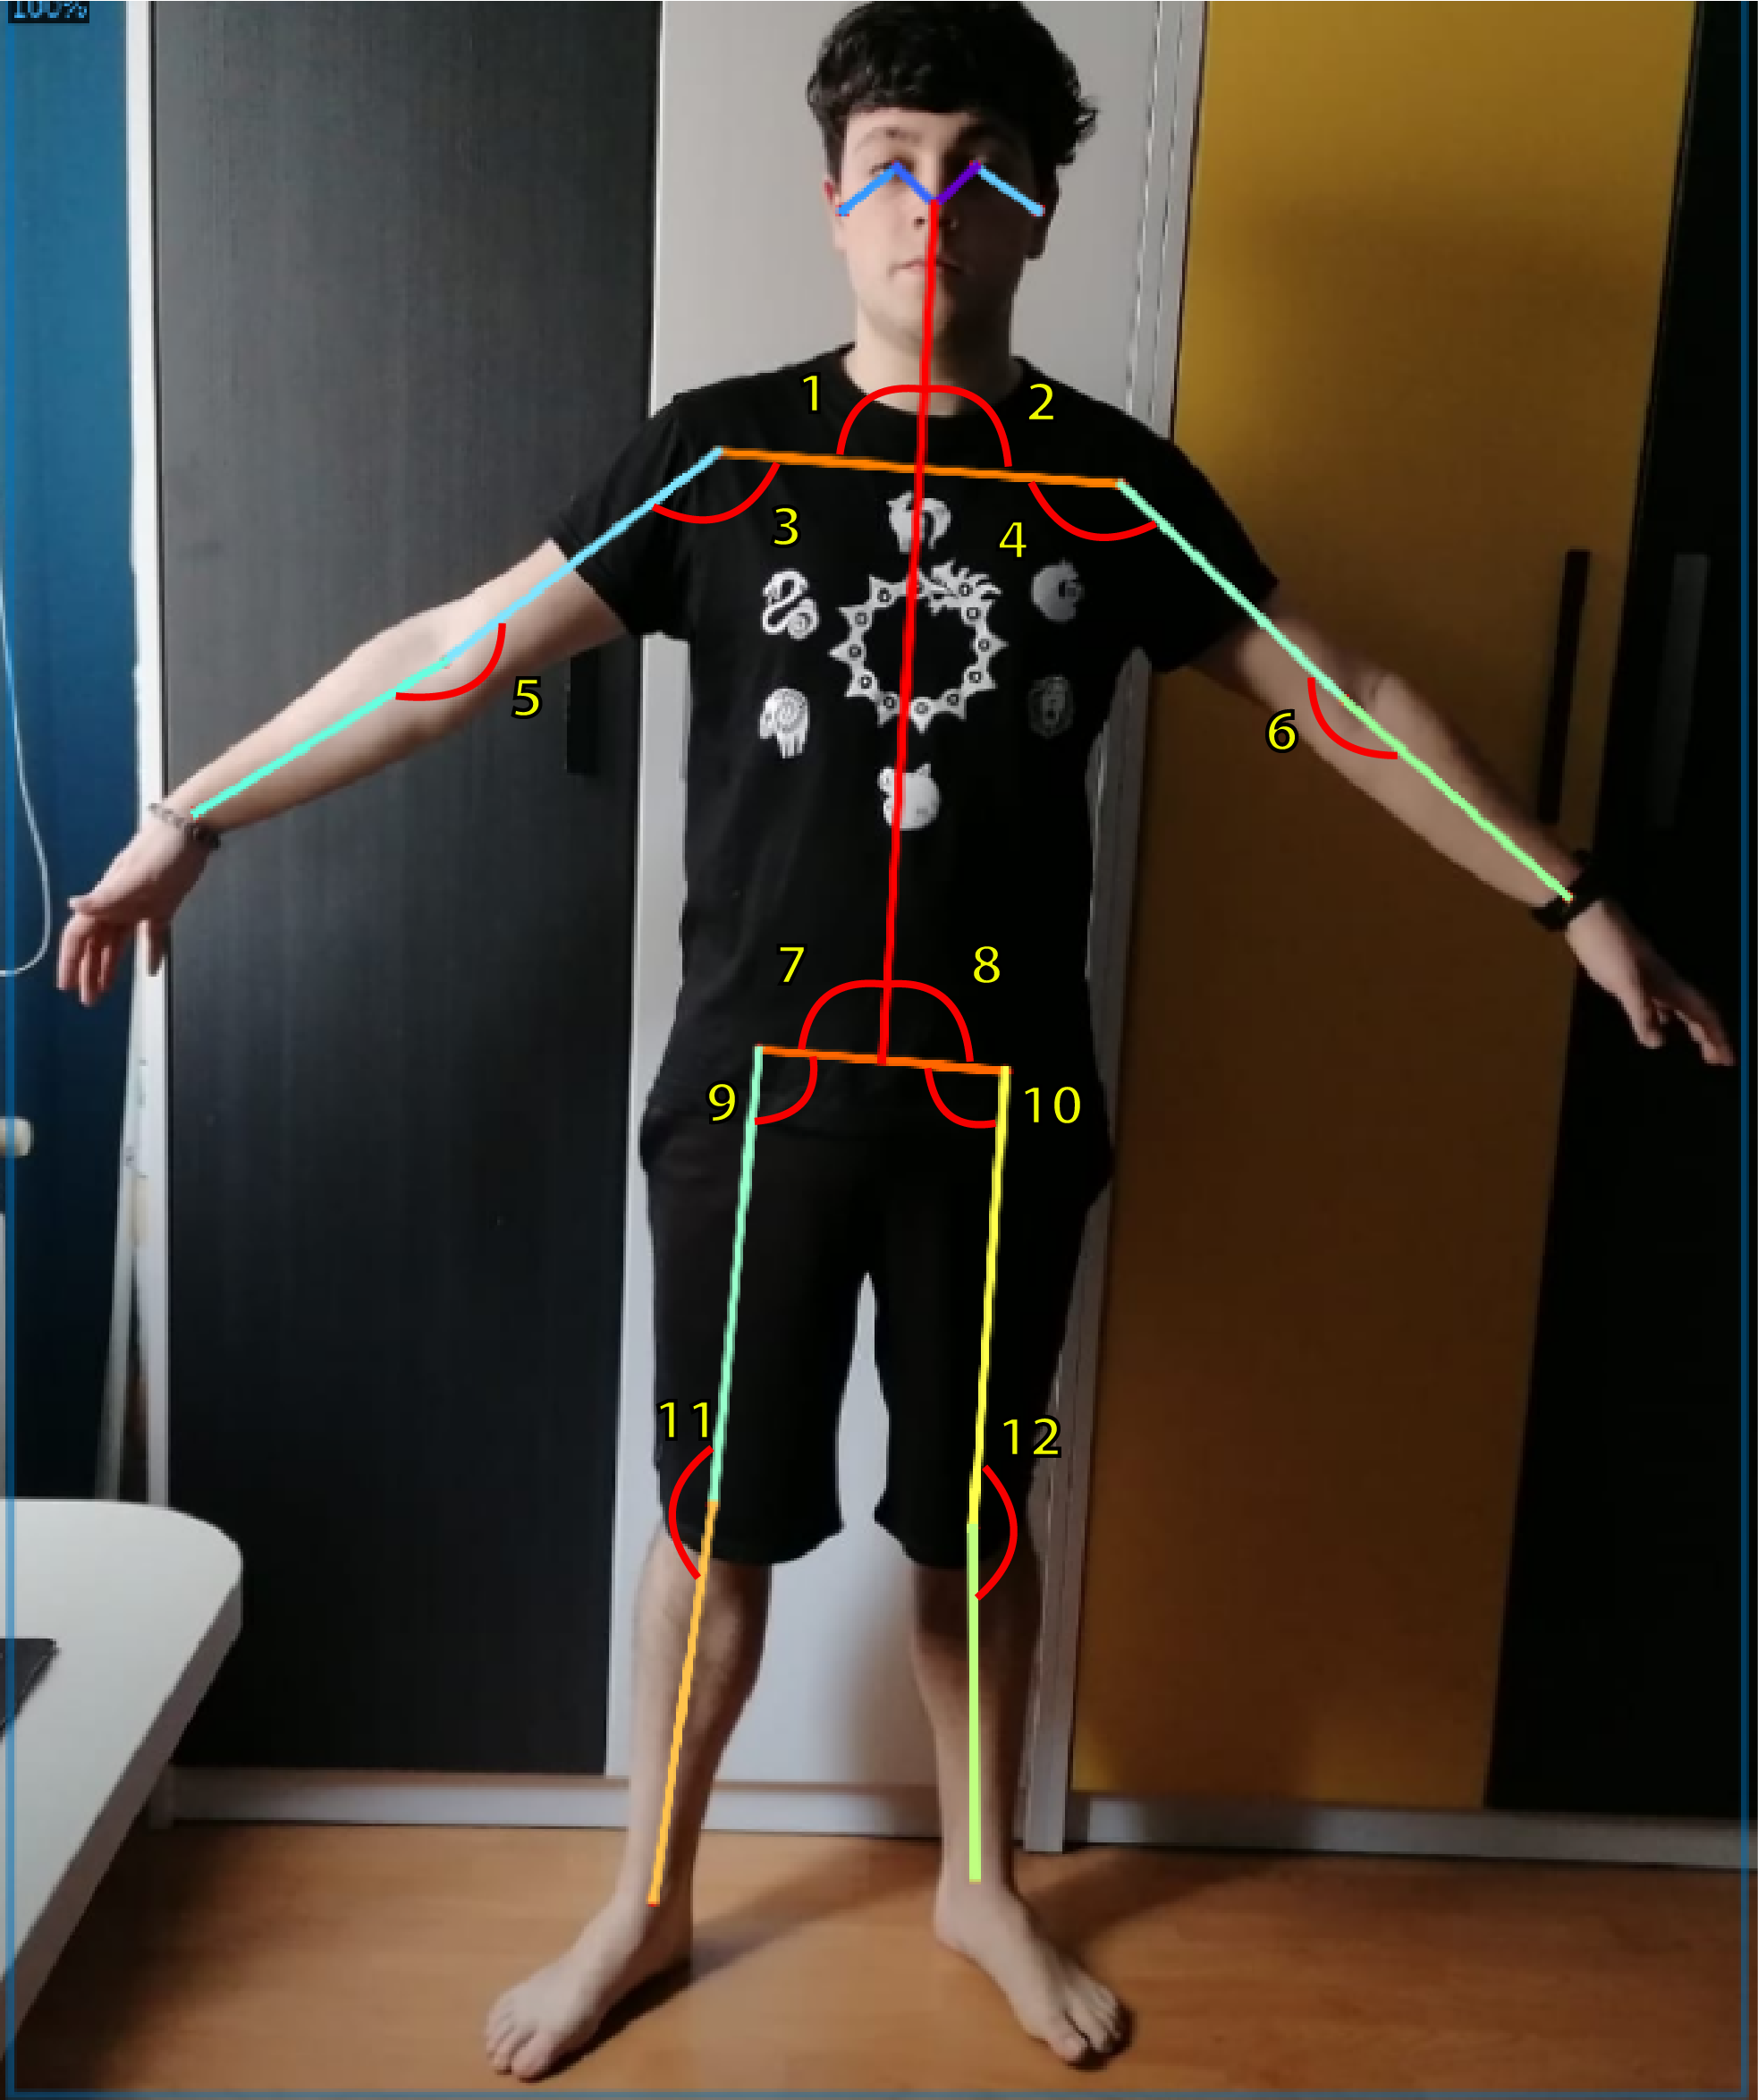
\includegraphics[width=0.5\textwidth]{estiradosAbajo2}
	\caption{Ejemplo ángulos sobre los que se calcula la diferencia entre posiciones.}
	\label{fig:estiradosAbajo2}
\end{figure}

La comparación de cada una de las partes se realiza calculando la suma de los valores absolutos de las restas de los valores entre las dos posiciones.

\subsection{Problema con los ángulos de los brazos}
Tras haber implementado la primera versión se realizaron unas pruebas para comprobar su funcionamiento. En esta pruebas se encontró un fallo muy importante, ya que los ángulos que se obtenían eran hasta 180 grados, ya que si se superaba este valor el ángulo se calculaba sobre el otro lado del punto central, es decir, nunca es superior a 180 grados. Es por ello que  posiciones como las que se pueden ver en las figuras~\ref{fig:brazosAbajo} y~\ref{fig:brazosArriba} tiene ángulos en ambos codos muy parecidos, aunque su posición sean casi contrarias.

\begin{figure}[h]
	\centering
	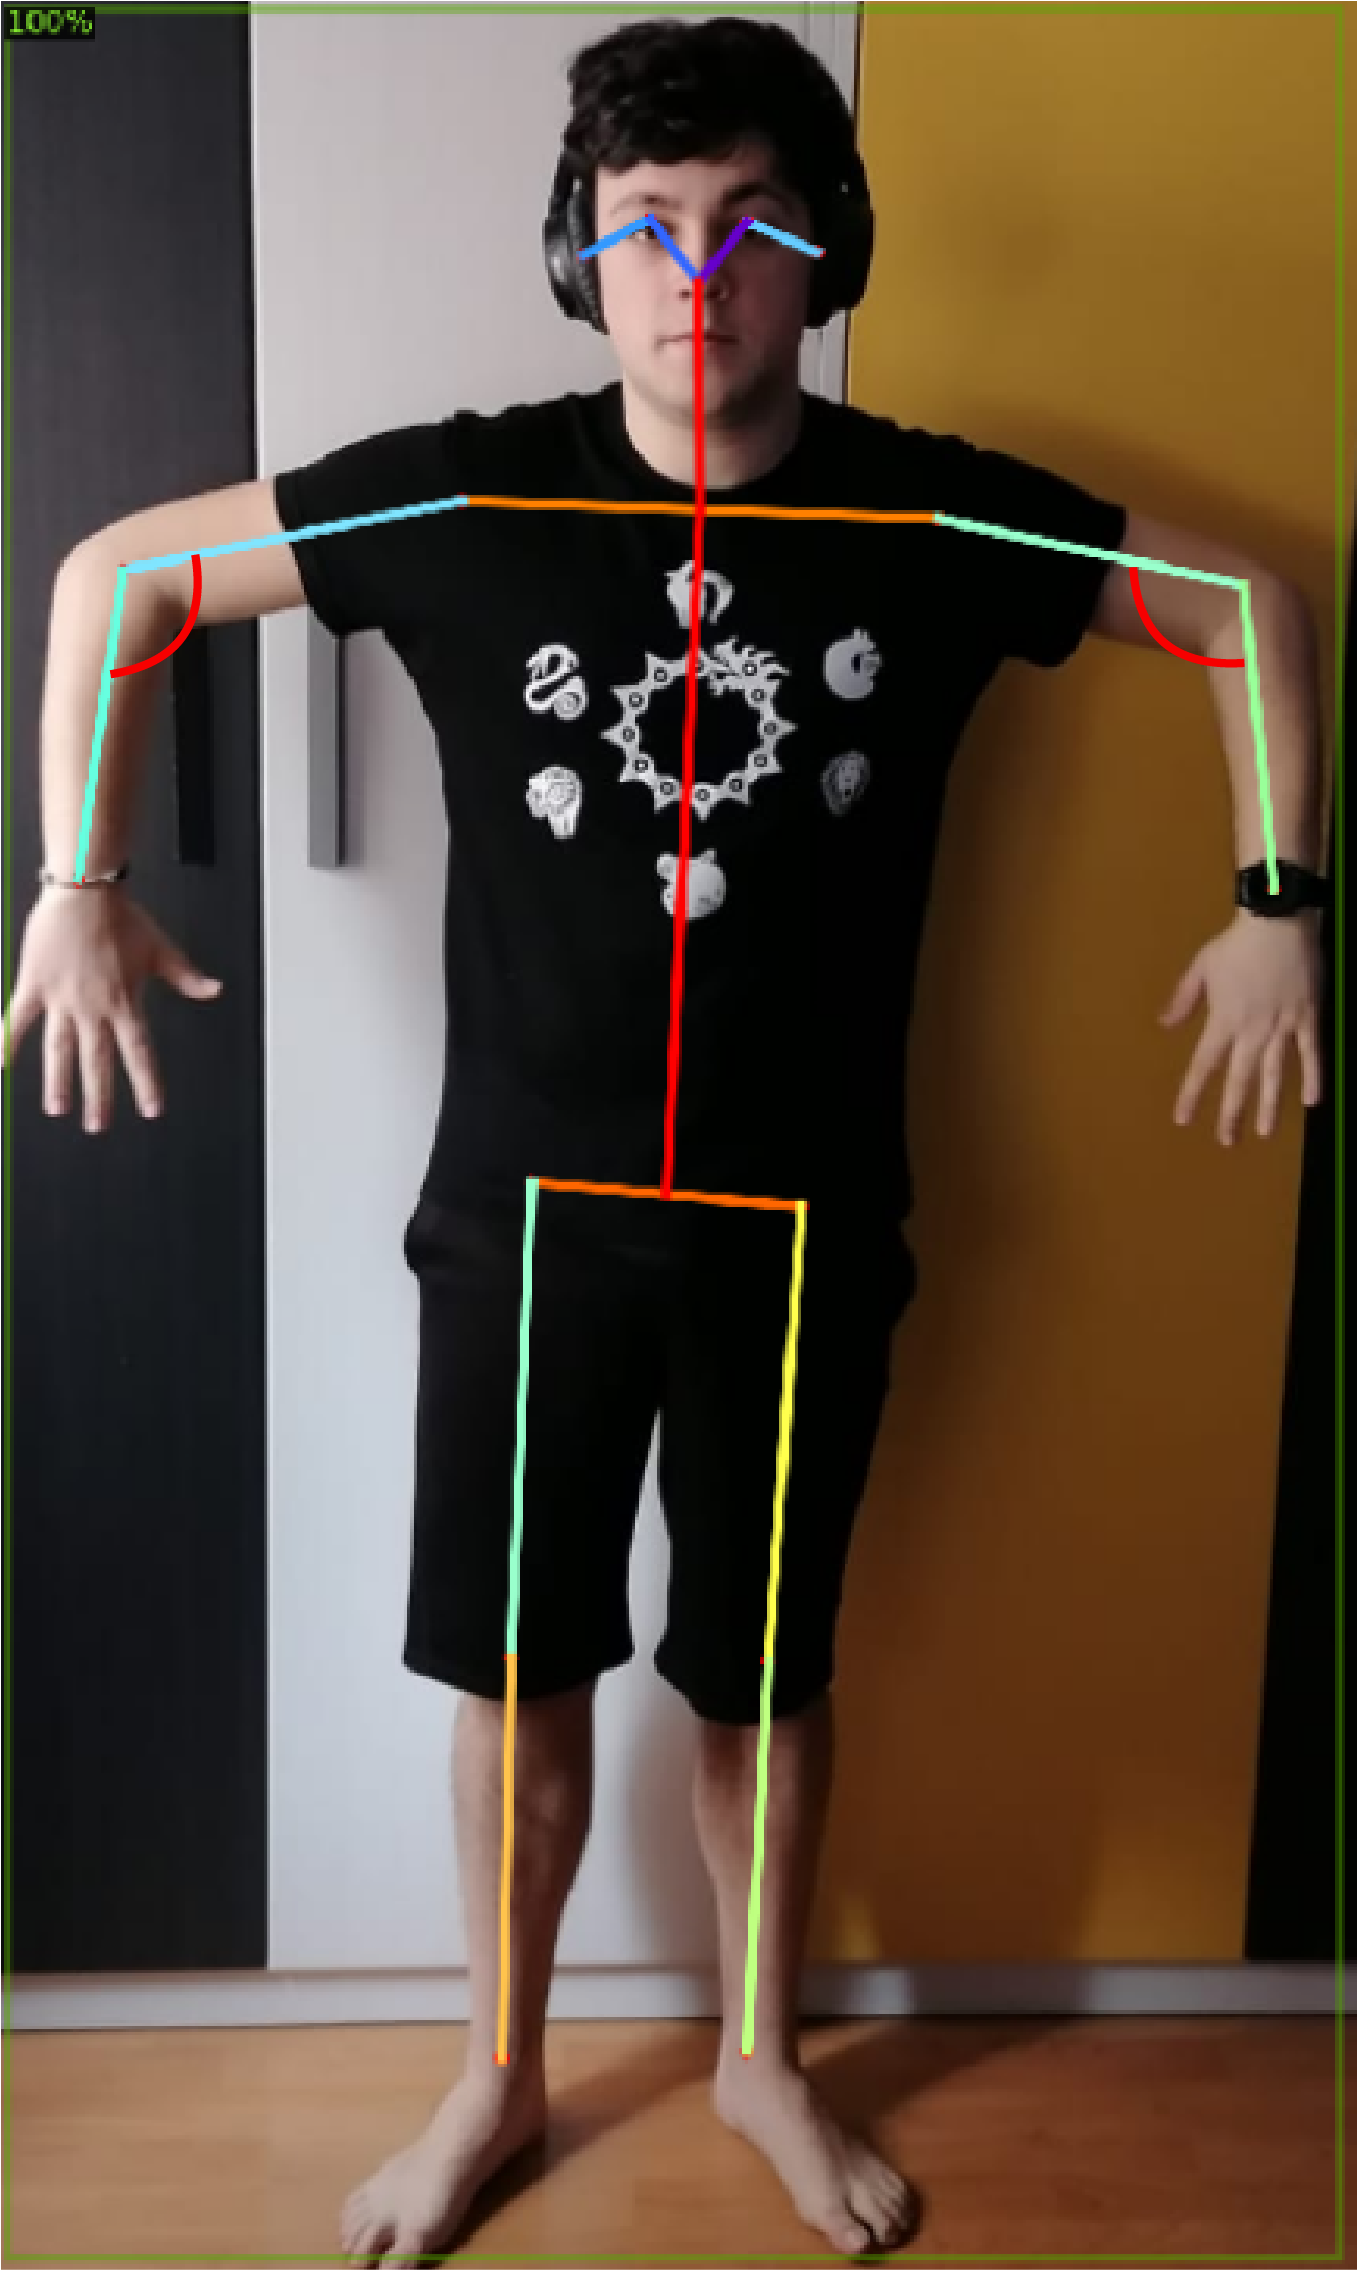
\includegraphics[width=0.5\textwidth]{brazosAbajo}
	\caption{Posición con los codos en 90 grados mirando hacia abajo.}
	\label{fig:brazosAbajo}
\end{figure}

\begin{figure}[h]
	\centering
	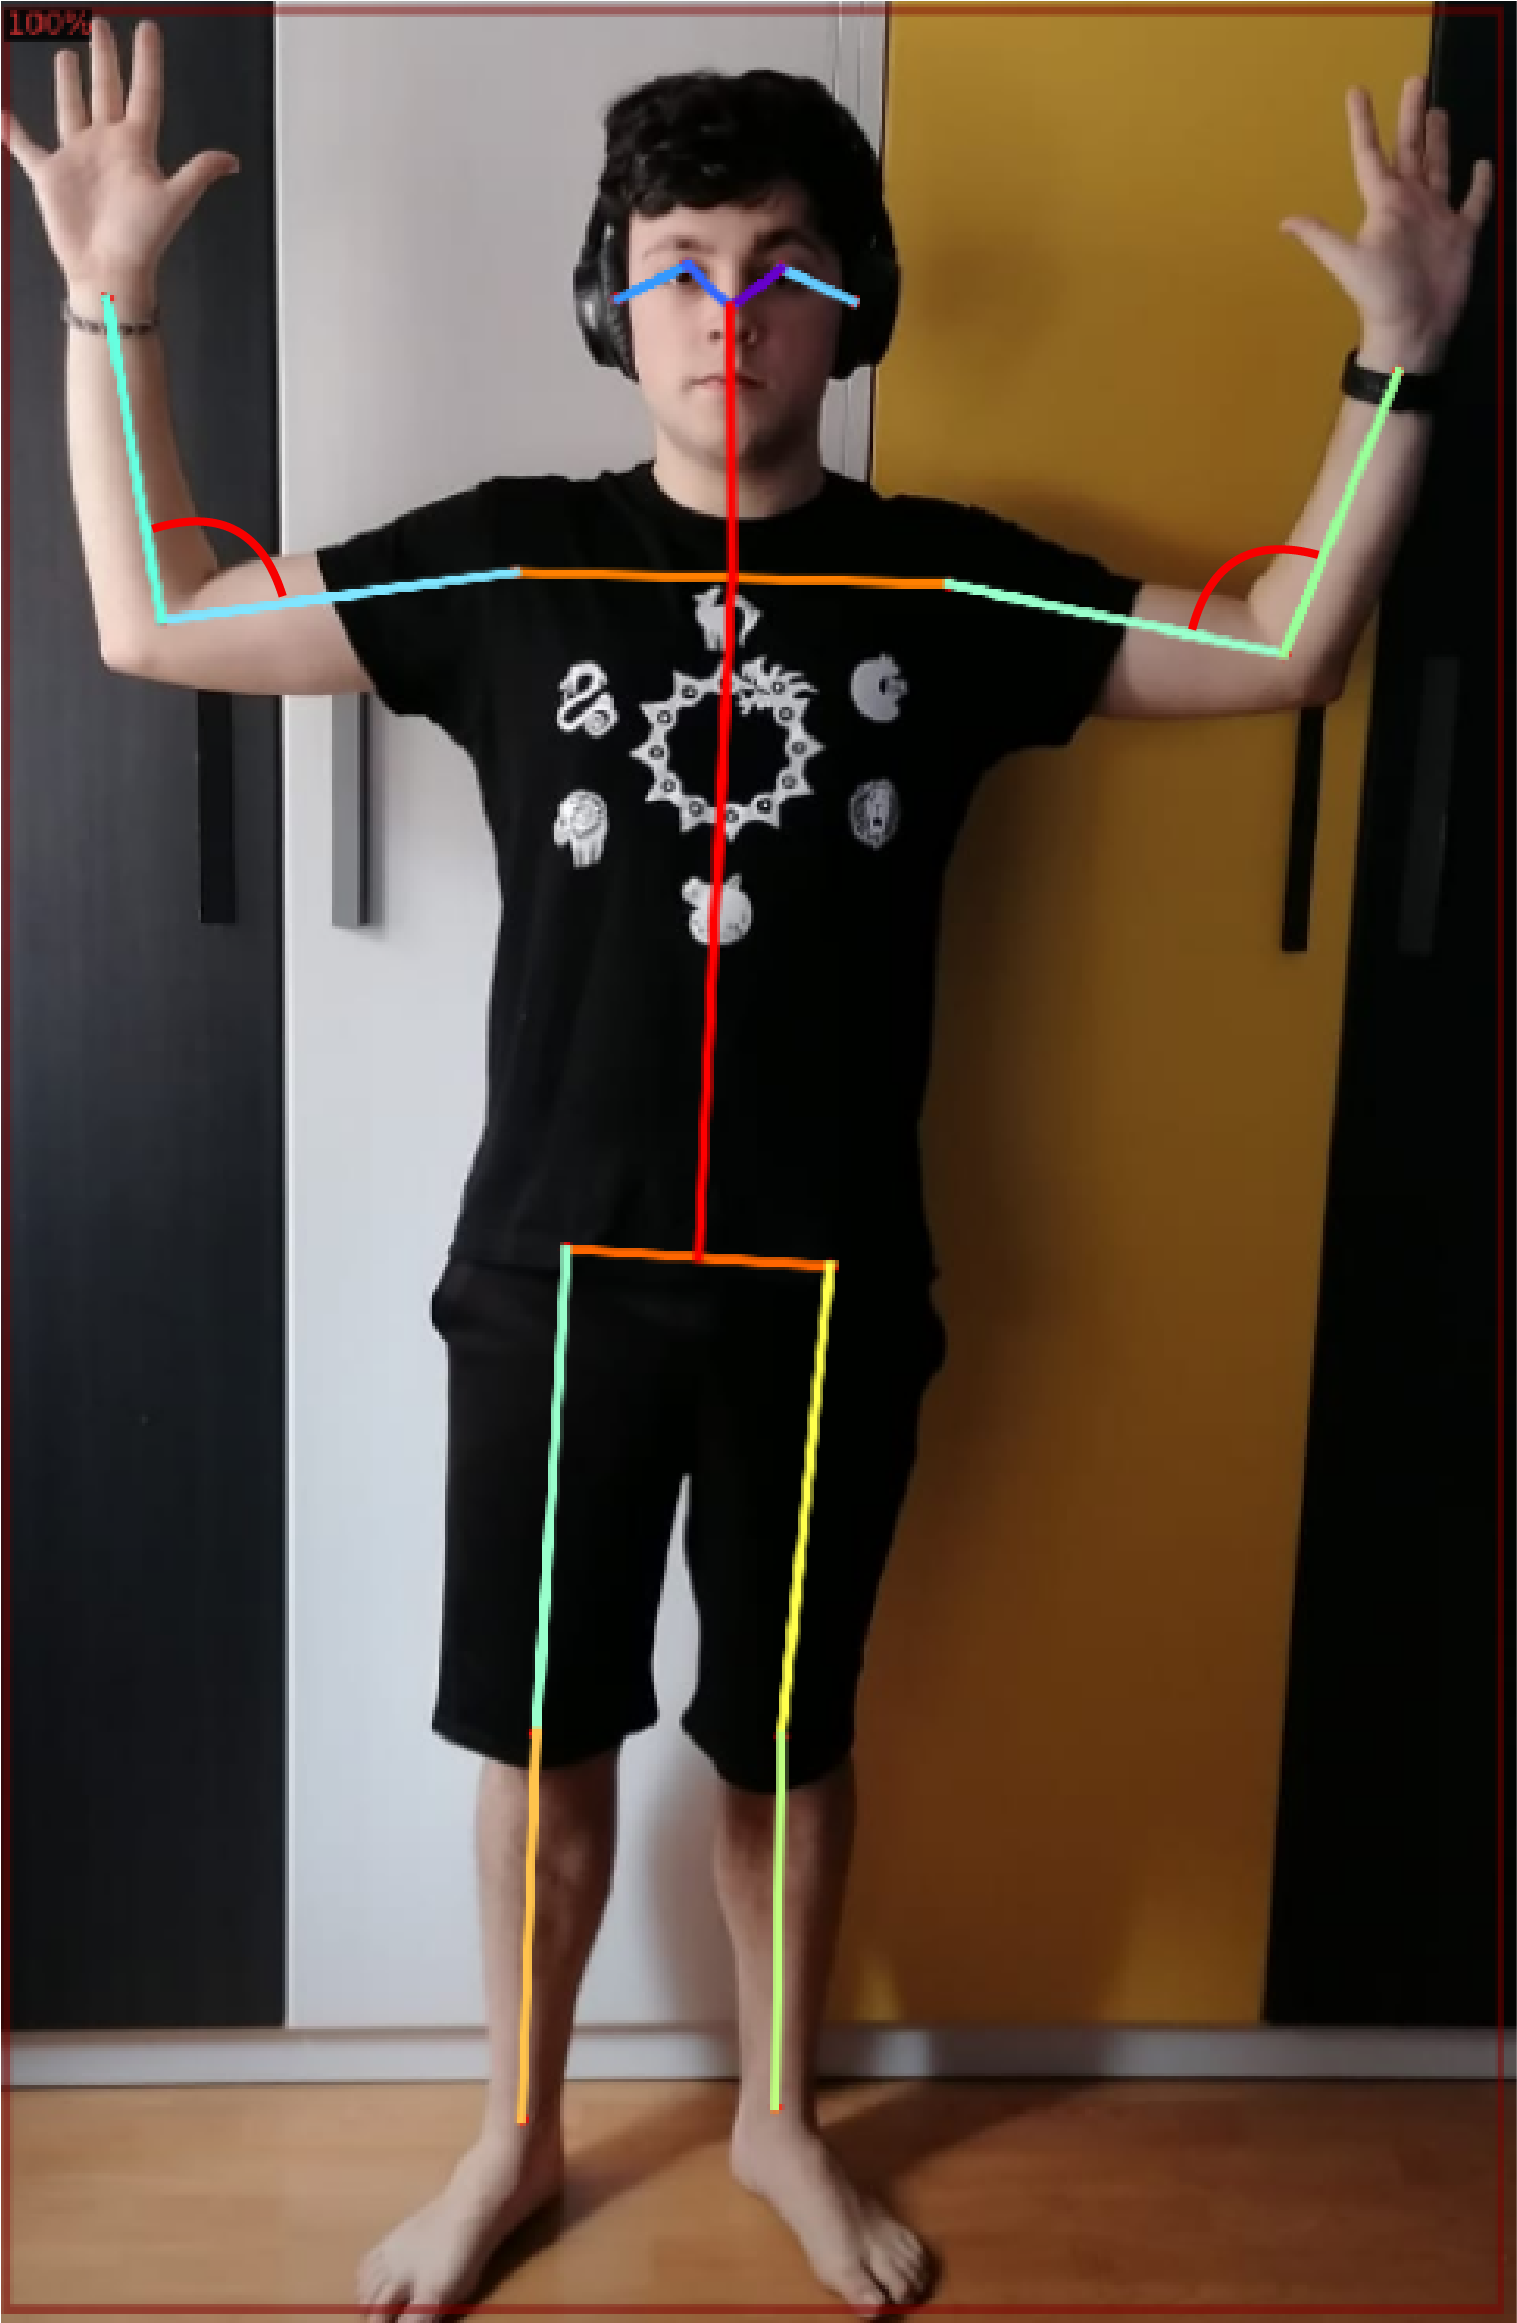
\includegraphics[width=0.5\textwidth]{brazosArriba}
	\caption{Posición con los codos en 90 grados mirando hacia arriba.}
	\label{fig:brazosArriba}
\end{figure}

Además, se descubrió que este error con los braozs se daba a demás de en los codos en los ángulos de los hombros, ya que posiciones como las que se pueden ver en las figuras~\ref{fig:estiradosAbajo} y~\ref{fig:estiradosArriba} obtienen ángulos muy parecidos, por la misma razón que pasaba con los codos.

\begin{figure}[h]
	\centering
	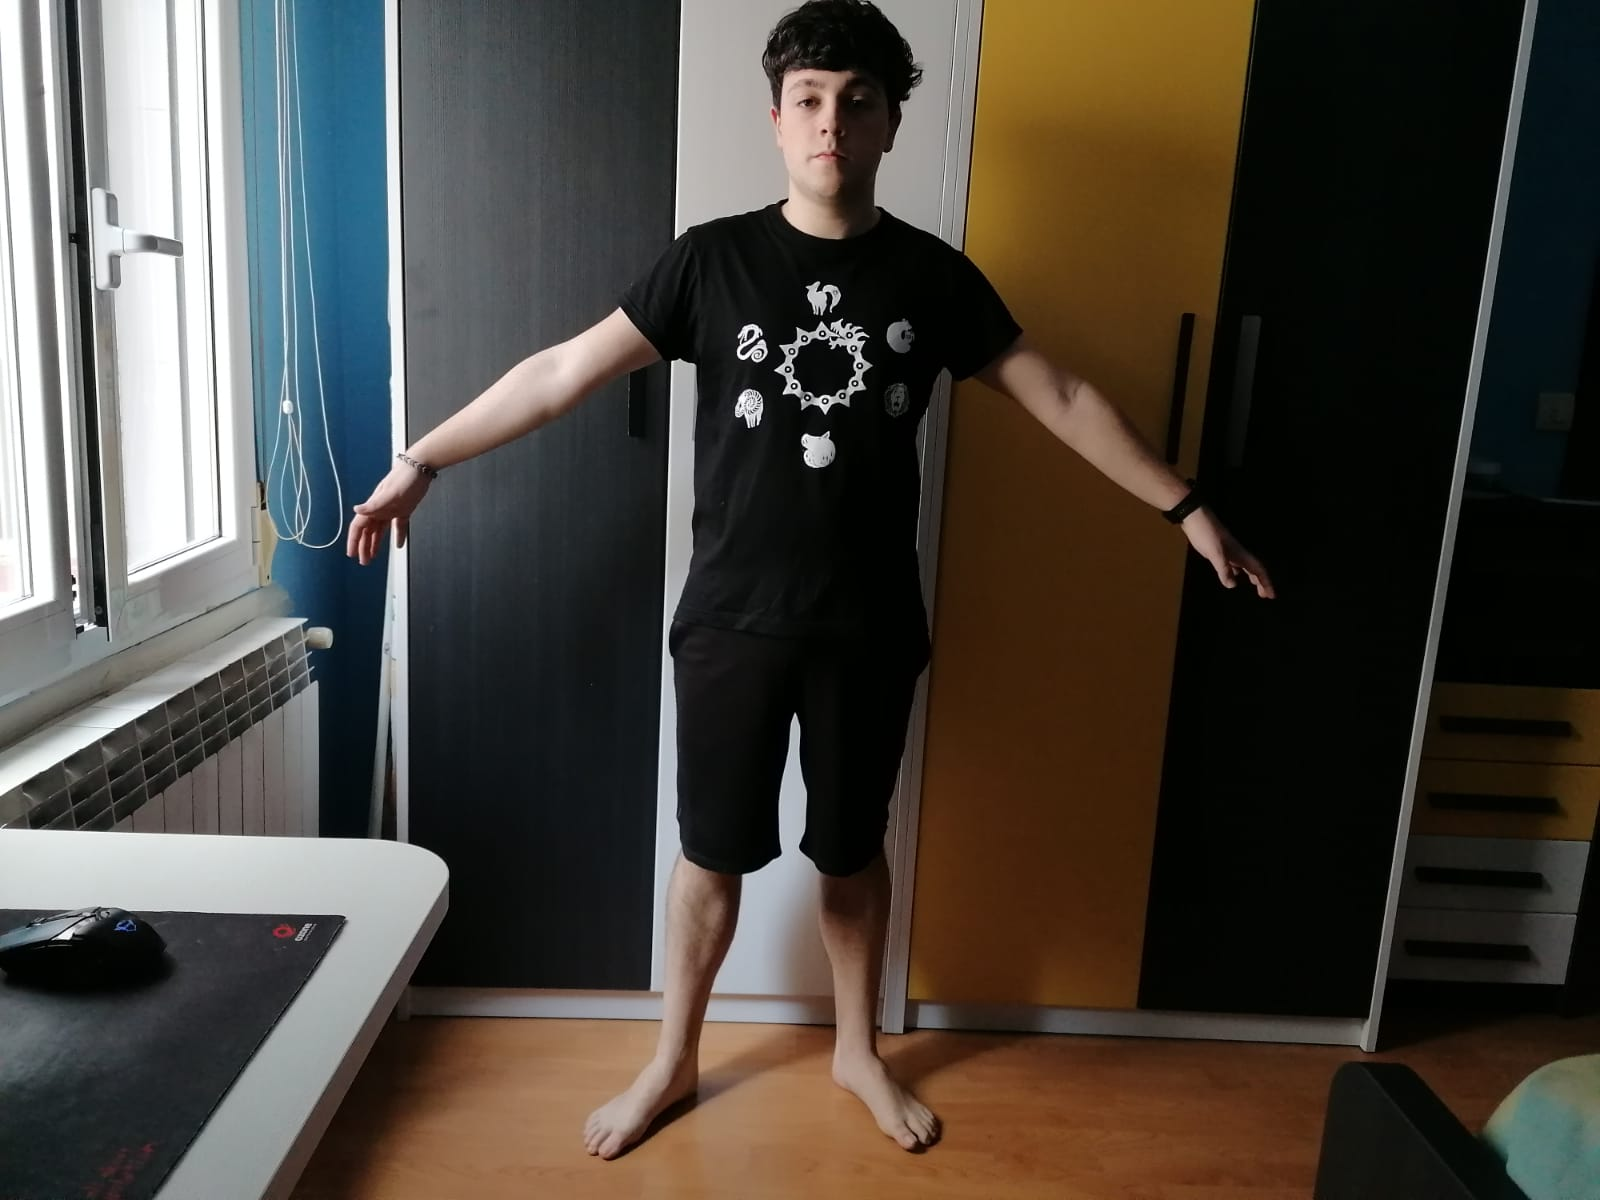
\includegraphics[width=0.5\textwidth]{estiradosAbajo}
	\caption{Posición con los hombros en 45 grados mirando hacia abajo.}
	\label{fig:estiradosAbajo}
\end{figure}

\begin{figure}[h]
	\centering
	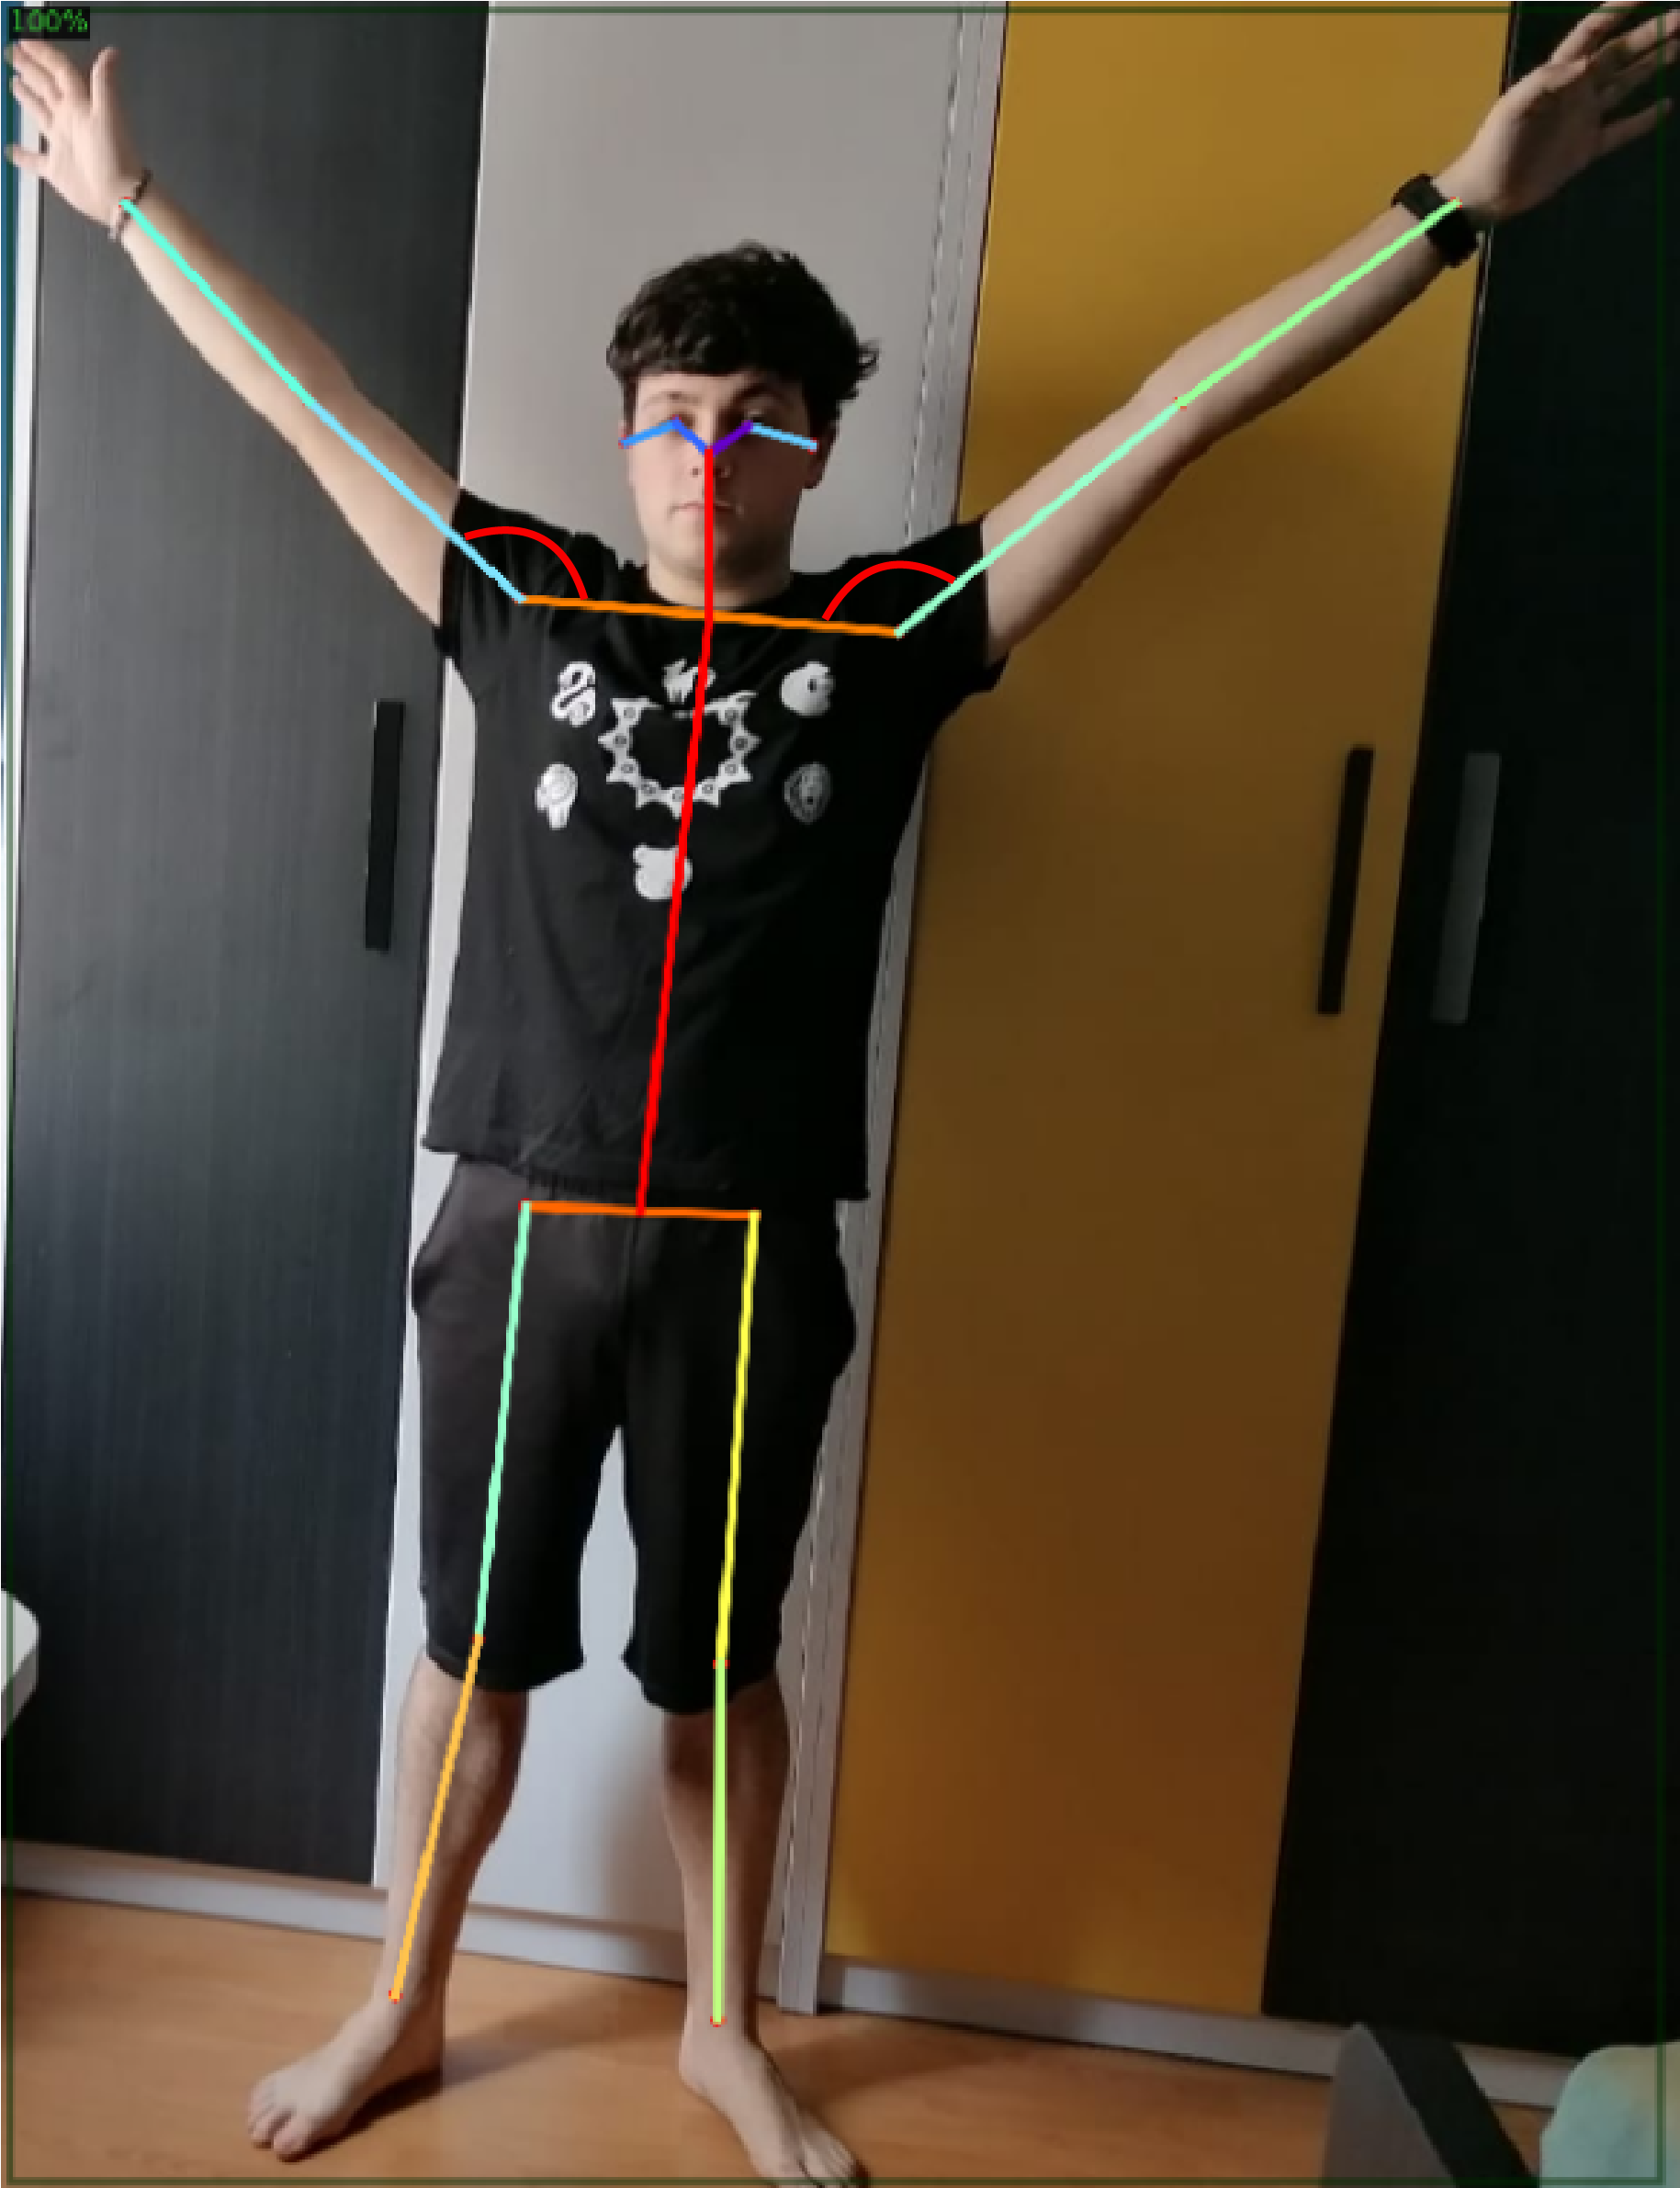
\includegraphics[width=0.5\textwidth]{estiradosArriba}
	\caption{Posición con los hombros en 45 grados mirando hacia arriba.}
	\label{fig:estiradosArriba}
\end{figure}

Para poder solucionar estos problemas lo primero que se hizo fue pasar los ángulos de los hombros que se encontraban en la comparación del torso a la comparación de los brazos. Después, para ambas partes se implemento el siguiente algoritmo para poder penalizar estos casos especiales:
\begin{enumerate}
	\item Comparar el ángulo (codo y hombro), si este está en un rango de 180 más menos un parámetro se dice que el codo u hombro está estirado y se le da el tipo 0.
	\item Si no está en tipo 0 se comprueba la altura del siguiente punto, en el caso del codo el siguiente punto es la muñeca, y en el caso del hombro el punto del codo. Se comprueba entonces si este segundo punto está por encima, y entonces se le da el tipo 1, sino se le da el tipo 2.
	\item Se comparan los tipos de las dos posiciones que se están comparando. Si cualquiera de las dos posiciones está estirada (tipo 0) entonces no se penaliza sea cual sea el tipo de la otra posición. Por el contrario, si ninguno de las dos posiciones tienen tipo 0, y sus tipos son distintos (uno tiene tipo 1 y le otro tipo 2) se penaliza sumando a la resta del absoluto de los ángulos un valor parametrizado, ya que se encuentran en posiciones muy distintas.
\end{enumerate}

Una vez se implementó esta nueva comparación para los brazos se realizaron una serie de imágenes de prueba para poder confirmar el correcto funcionamiento de la nueva implementación.

\subsection{Umbral y penalización}
Como se ha comentado, en esta segunda versión, que se centró en el problema con los brazos, se han utilizado dos parámetros un umbral para definir el rango en el que se considera que un ángulo está estirado o no, y la penalización que se aplica si los tipos son distintos.

Al principio se puso un umbral de 10 grados, que para las imágenes de pruebas que se obtuvieron se recogieron buenos resultados, diferenciando correctamente cuando una de las partes estaba o no estirada. Lo mejor de que este valor sea un parámetro es que se puede modificar dependiendo del ejercicio a realizar.

Por otro lado, al implementar la penalización se utilizó el mismo valor tanto para los codos como para los hombros, con una valor de 180 grados de penalización. Pero en comprobaciones que se realizaron después se observó que penalizar a los hombros con el mismo valor que a los codos no era correcto, ya que la diferencia no era tan grande. Es por ello que se dividió este parámetro de penalización en dos, uno para los codos a 180 y otro para los hombros a 90. Aun así, como pasa con el umbral, estos valores se puede modificar dependiendo del ejercicio a comparar.

\section{Versión 3 de comparación, uso de medias}
Una vez se creía que la comparación de posiciones era correcta había que dar sentido a los valores obtenidos. La forma que se encontró más oportuna para poder realizar esta operación fue el uso de la media de los valores obtenidos en las distintas zonas con las que se trabaja (brazos, piernas y torso).

Además, se implementó el cálculo de la media de tal manera que al aplicar los distintos pesos a las zonas el valor final obtenido siguiese siendo un valor entre 0 y 180 (la distancia máxima que puede haber entre dos ángulos).

Teniendo esto en cuenta el resultado final se calcula con la siguiente fórmula (siendo $total$ la suma de los tres pesos):
\begin{equation}
\begin{split}
resultado = (pesoBrazos/total)*compBrazos +\\ (pesoPiernas/total)*compPiernas (pesoTorso/total)*compTorso
\end{split}
\end{equation}

\section{Error en brazos, nueva posición y comparación}
Una vez se creía que se tenía una versión final para la comparación de posiciones, ya que las pruebas con las imágenes que antes daban problemas se daba un buen resultado, se probó con lo vídeos que se habían grabado en la primera recogida de datos de prueba. En esta segunda prueba sobre esta versión se encontró un error muy grave, ya que se penalizaban situaciones en los brazos que nunca se deberían de penalizar.

Estos casos donde se penalizaban eran cuando las manos pasaban de estar por encima de los codos a pasar por debajo, o viceversa. Un ejemplo de esta situación se puede ver en la figura~\ref{fig:errorbrazos}, donde se la diferencia en los brazos entre las dos imágenes se debería calcular únicamente con la diferencia de los ángulos de los codos, pero que con la implementación de la versión 3, además de la diferencia entre los ángulos, se sumaría una penalización de 180 grados a la diferencia.

\begin{figure}[h]
	\centering
	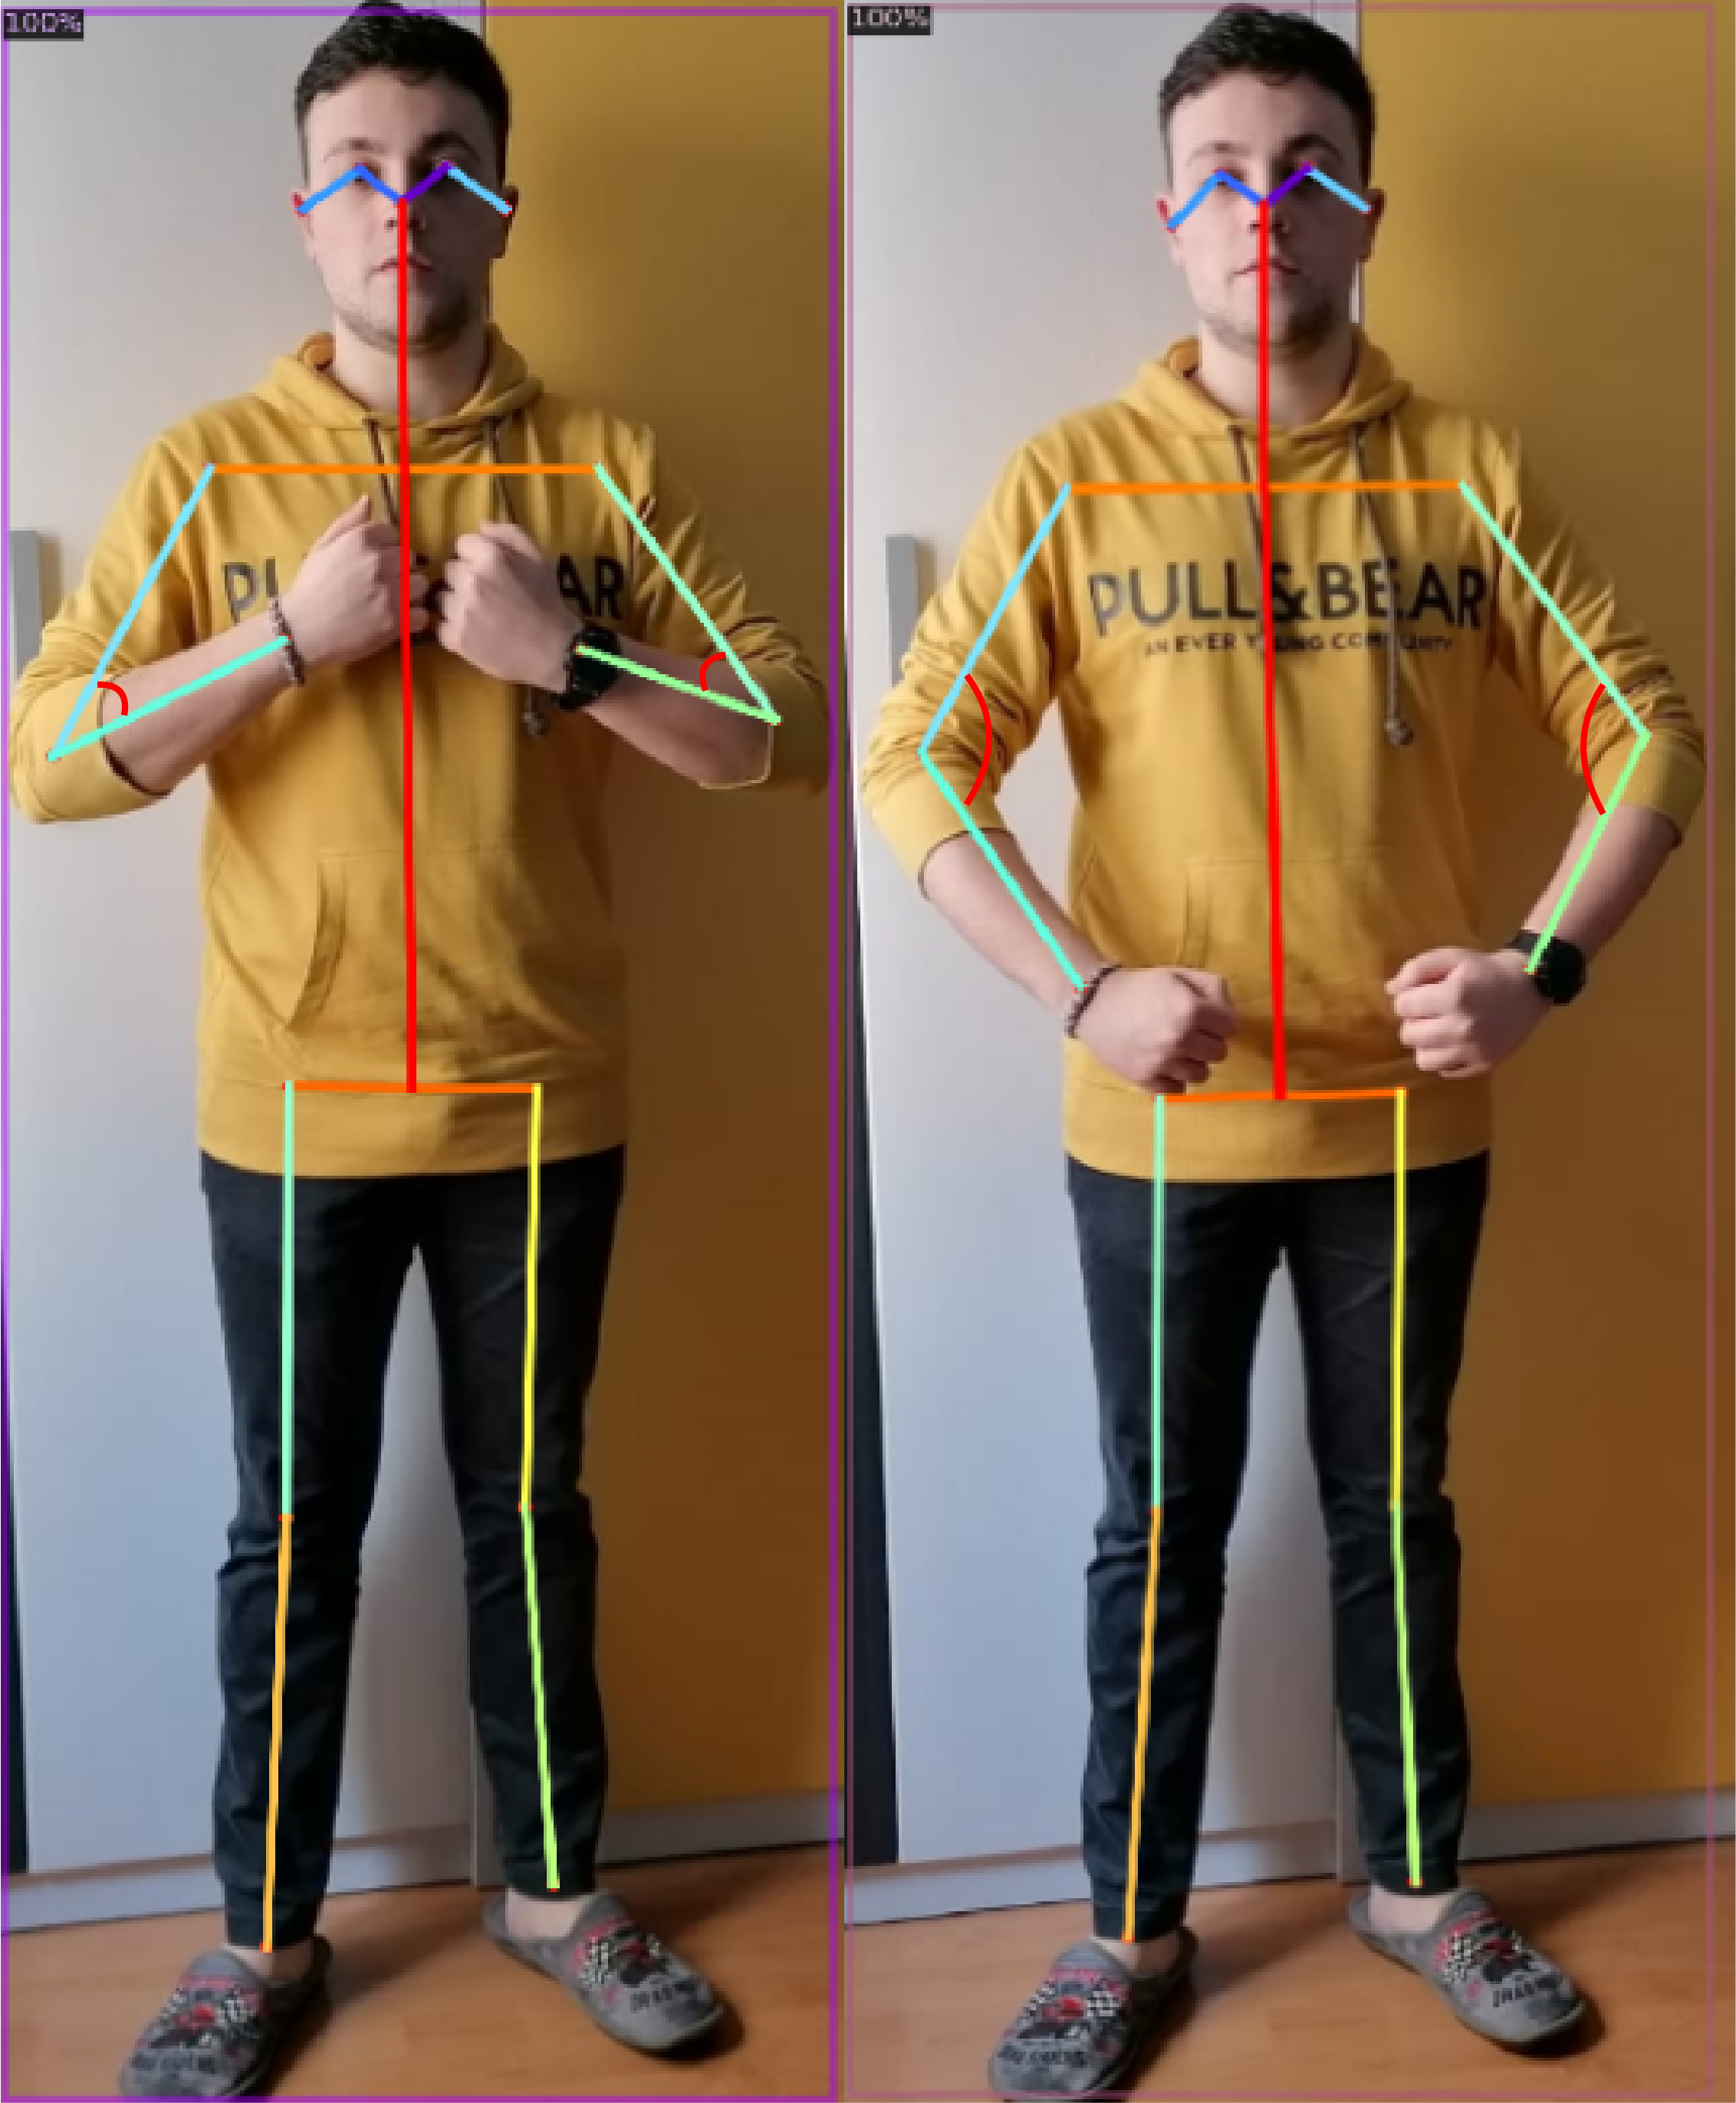
\includegraphics[width=0.5\textwidth]{errorbrazos}
	\caption{Ejemplo de error en la comparación de brazos.}
	\label{fig:errorbrazos}
\end{figure}

En esta situación, se plantearon una serie de posibles soluciones a este problema ya reincidente. Primero se intentó dar solución al problema manteniendo el sistema de la posición y el resto de comparaciones que daban errores, pero no se ideó una solución plausible que solucionara todos los problemas encontrados en las diversas versiones de la comparación de posiciones. Es por ello que se pasó a hacer una cambio más radical, subiendo a un nivel superior el problema, a la clase de \textit{Python} de la posición.

\subsection{Nueva versión clase posición}

En la primera versión de esta clase, los ángulos se calculaban de forma que nunca eran superiores a 180 grados, lo que daba la necesidad de penalizar ciertas situaciones.

En la segunda versión de la clase se eliminó la condición de que los ángulos fuesen solo de 180 grados (salvo para los ángulos del cuello y de la cadera con el torso, ya que estos ángulos no pueden ser mayores de 180 por fisionomía humana). Para poder expresar el ángulo en un rango de 360 grados se implementó el siguiente algoritmo que utiliza la función anterior de cálculo del ángulo entre 3 puntos:

\begin{lstlisting}[language=Python]
#p1,p2,p3: puntos a calcular el angulo,
# p2 debe ser el punto central
#lado: 0 izquierda, 1 derecha
def calcularAngulo(self,p1,p2,p3,lado):
     flag=False
     ang = self.calcularAuxAngulo(p1,p2,p3)
     
     #Cuando la recta que une los dos primeros
     # puntos es una linea vertical
     if (p2[0]-p1[0]) ==0:
         
         #Lado derecho
         if lado:
             #Si la posicion esta menos a la derecha 
             #se ha de cambiar el angulo
             if p3[0]<p2[0]:
                 flag=True
         
         #Lado izquierdo
         else:
             #Si la posicion esta menos 
             #a la izquierda se ha de cambiar el angulo
             if p3[0]>p2[0]:
                 flag=True
         
         #Cambio del angulo
         if flag:
             ang = 360 - ang
     else:
         #Calculo de la ecuacion de la recta sustituyendo
         # el valor de x por el valor del tercer punto
         y = ((p2[1]-p1[1])*(p3[0]-p1[0])/(p2[0]-p1[0]))+p1[1]
         
         #Si esta la tercera parte por encima de la recta que 
         #hacen las dos primera entonces se cambia el angulo
         if p3[1] > y:
             ang = 360 - ang
     
     return ang
\end{lstlisting}

Los pasos que sigue este algoritmo es:
\begin{enumerate}
	\item Calcular el ángulo en un rango de 180 grados, con la implementación de la anterior versión de la clase de la posición.
	\item Comprobar si los dos primeros puntos, de los tres estudiados, forman una línea vertical comprobando la resta en sus valores del eje x. Si som iguales ir a 3, sino ir a 4.
	\item Si los dos puntos forman una línea vertical no tiene sentido comparar la altura con el tercer punto. Es por ello que lo que se hace es comprobar, dependiendo del lado (izquierda o derecho), la posición del tercer punto analizando si este este más cercano eal centro del cuerpo (el ángulo se mantiene igual), o si por el contrario está más al exterior del cuerpo donde se realiza una resta de 360 grados menos el ángulo calculado.
	\item Si por el contrario los dos puntos no están en una línea vertical (caso más común) se calcula la ecuación de la recta con estos dos primeros puntos. En esta ecuación de la recta se sustituye el valor de x por el valor de este eje del tercer punto. Por último se comprueba si el valor de y calculado con la ecuación de la recta sustituyendo la x es superior (se mantiene el ángulo) o inferior al valor y del tercer punto donde habría que cambiar el valor del ángulo por 360 menos el ángulo calculado al principio del algoritmo.
	\item Se devuelve el valor calculado del ángulo.
\end{enumerate}

\subsection{Nueva versión comparación}
Una vez se había modificado la clase de la posición era necesario hacer una serie de cambios en la comparación de éstas. En este caso, al realizar estos cambios, ya hacía falta <<discriminar>> la comparación de los brazos, ya que ahora todos se calculan de la misma forma y no se necesita ningún umbral ni penalización. Además, aprovechando que no había que realizar ninguna discriminación, por la zona que se estuviese comparando, se realizó una factorización del código implementado para reducir el código repetido.

Para esta cuarta versión de la comparación de las posiciones se realizaron dos funciones. La primera función permite el cálculo de la media de la diferencia entre los ángulos de las zonas pasadas. El código de esta función se puede ver a continuación:

\begin{lstlisting}[language=Python]
#pos1,pos2: posiciones a comparar
#zonas: lista de las zonas a comparar
# zonas sin especificar la parte izq o drch
def comparacionZona(pos1,pos2,zonas):
	#Partes derecha e izquierda
	partes=["D","I"]
	#Resultado iniciado a 0
	res = 0.0
	
	#Recorrer las partes
	for i in partes:
		#Recorrer las zonas
		for j in zonas:
			#aux es la diferencia entre los angulos
			aux = abs(eval("pos1."+j+i)-eval("pos2."+j+i))
	
			#Si la diferencia es mayor de 180
			# grados se coge el otro lado para
			# mantener la distancia minima
			if aux > 180:
				res += (360-aux)
			else:
				res+=aux
	
	#Se devuelve el valor final entre el
	#numero de elementos sumados
	return res/(len(partes)*len(zonas))
\end{lstlisting}

Como se puede ver en el código, esta implementación permite la comparación de todas las zonas de la posición y siempre devuelve una diferencia media entre las zonas comparadas que nunca supera los 180 grados, es decir, siempre devuelve la distancia mínima entre los ángulos.

Pero para poder dar distintos pesos a las distintas zonas a comparar se implementó la segunda función que llama a la función anterior, \texttt{comparacionZona}. El código de esta función final que devuelve la diferencia media aplicando los pesos se puede ver a continuación:

\begin{lstlisting}[language=Python]
#pos1,pos2 posiciones a comparar
#pesos: diccionario con los pesos de
# cada zona
def compararPosiciones(pos1,pos2,pesos={"brazos":1,
										"piernas":1,
										"torso":1}):
    zonas={"brazos":["angCodo","angHombro"],
    	  "piernas":["angRodilla","angCadera"],
    	  "torso":["angCaderaTorso","angCuelloSup"]}
    res=0
    total=0
    
    #Se recoge el peso total
    for i in pesos:
    	#Si no esta en las keys de la zona se lanza
    	# una excepcion
        if i not in zonas:
            raise Exception("Excepcion")
        total+=pesos[i]
        
    #Se recorren los distintos tipos de zonas
    # y se les aplica el peso a la comparacion
    for i in zonas:
        res+=(pesos[i]/total)*
        	 comparacionZona(pos1,pos2,zonas[i])

	#Calculo del porcentaje entorno a 180
    porcentaje = res*100/180
 
    return res,100-porcentaje
\end{lstlisting}

Como se puede ver en el código, la implementación recorre las distintas zonas de las cuales calcula la comparación entre las posiciones y le aplica el peso considerado. Además, una vez calculada la diferencia final, al estar está entre 0 y 180 grados por utilizar las medias, se calcula el porcentaje inverso de exactitud entre las dos posiciones. Este porcentaje se interpreta como el porcentaje de exactitud entre las posiciones, siendo el 100\% el valor máximo donde las dos posiciones son totalmente iguales.

\section{Comprobación de la última versión}
Una vez se terminó de implementar estas nuevas versiones se probaron con las imágenes de la sección~\ref{PrimeraVersion} que la implementación funcionaba correctamente con los datos que las primeras dos versiones tenían grandes problemas. Después, para poder probar el funcionamiento y sobre todo el rendimiento de la implementación se desarrolló unas funciones que permiten recorrer todos los vídeos de una carpeta y de cada vídeo comparar un fotograma con el siguiente de ese mismo vídeo (objetivo principal del proyecto). Cabe comentar en que esta comparación se ha dado el mismo peso a todas las zonas comparadas. Gracias a estas funcionas se pudo obtener los siguientes datos de cada uno de los vídeos:
\begin{itemize}
	\item Media de la diferencia de los grados en todo el vídeo.
	\item Diferencia máxima en grados en todo el vídeo.
	\item Diferencia mínima en grados en todo el vídeo.
	\item Desviación típica entre las diferencias de los grados.
	\item Media del porcentaje de exactitud.
	\item Porcentaje máximo de exactitud.
	\item Porcentaje mínimo de exactitud.
	\item Desviación típica de los porcentajes.
	\item Número de fotogramas en el vídeo.
	\item Tiempo de obtención de las posiciones del vídeo.
	\item Tiempo de comparación de las posiciones del vídeo.
	\item Tiempo de cálculo de estadísticas de las comparaciones del vídeo.
	\item Tiempo total.
	\item Tiempo total empleado por fotograma.
\end{itemize}

Los resultados obtenidos en esta fase se pueden ver en:
\begin{itemize}
	\item Resultados diferencia en grados: tabla~\ref{tab:difgra}.
	\item Resultados diferencias en porcentajes: tabla~\ref{tab:difpor}.
	\item Resultados tiempos de ejecución: tabla~\ref{tab:tiempos}.
\end{itemize}

\begin{table}[h]
	\centering
	\resizebox{\columnwidth}{!}{
\begin{tabular}{lrrrr}
	\toprule
	Vídeo &  MediaGrados  &  GradosMáximos &  GradosMínimos &  DesviaciónGrados \\
	\midrule
	depie &     $5.26$ &      $34.89$ &       $0.46$ &          $5.93$ \\
	sentado1 &     $2.68$ &      $26.07$ &       $0.05$ &          $3.01$\\
	sentado6-camiseta &     $2.36$ &       $5.27$ &       $0.32$ &          $0.96$\\
	sentado2-cruzado-480 &     $2.74$ &      $14.59$ &       $0.58$ &          $1.72$\\
	sentado4-remangado &     $2.78$ &      $23.80$ &       $0.22$ &          $2.96$\\
	sentado2-cruzado &     $2.79$ &      $15.35$ &       $0.40$ &          $1.81$\\
	sentado3-caja &     $2.62$ &      $34.32$ &       $0.15$ &          $4.13$\\
	sentado5-chaqueta-abierta&     $2.96$ &      $17.29$ &       $0.42$ &          $1.94$\\
	\bottomrule
\end{tabular}
}
\caption{Tabla con las estadísticas de las diferencias en grados.}
\label{tab:difgra}
\end{table}

\begin{table}[h]
	\centering
	\resizebox{\columnwidth}{!}{
\begin{tabular}{lrrrr}
	\toprule
	Vídeo&  PorcMedio &  PorcMáximo &  PorcMínimo &  DesvPorcentaje\\
	\midrule
	depie&        $97.08$ &         $99.74$ &         $80.61$ &              $3.29$\\
	sentado1 &        $98.51$ &         $99.97$ &         $85.52$ &              $1.67$\\
	sentado6-camiseta &        $98.69$ &         $99.82$ &         $97.07$ &              $0.53$\\
	sentado2-cruzado-480 &       $98.48$ &         $99.68$ &         $91.89$ &              $0.95$\\
	sentado4-remangado &       $98.46$ &         $99.88$ &         $86.78$ &              $1.65$\\
	sentado2-cruzado &        $98.45$ &         $99.78$ &         $91.47$ &              $1.01$\\
	sentado3-caja &        $98.54$ &         $99.92$ &         $80.93$ &              $2.29$\\
	sentado5-chaqueta-abierta &        $98.35$ &         $99.76$ &         $90.39$ &              $1.08$\\
	\bottomrule
\end{tabular}
}
\caption{Tabla con las estadísticas de las diferencias en porcentajes de exactitud.}
\label{tab:difpor}
\end{table}

\begin{table}[h]
	\centering
	\resizebox{\columnwidth}{!}{
		\begin{tabular}{lrrrrrr}
	\toprule
	Vídeo&  NFrames &  TiempoObtPos (s) &  TiempoComp (s) &  TiempoEst (s) &  TiempoTotal (s) &  Tiempo/Frame \\
	\midrule
	depie&$258$ &          $26.704819$ &           $0.045619$ &            $0.000168$ &    $26.750605$ &      $0.103685$ \\
	sentado1&$445$ &          $49.113378$ &           $0.075400$ &            $0.000146$ &    $49.188924$ &      $0.110537$ \\
	sentado6-camiseta&$194$ &          $21.433898$ &           $0.027136$ &            $0.000100$ &    $21.461134$ &      $0.110624$ \\
	sentado2-cruzado-480&$286$ &          $31.532470$ &           $0.039944$ &            $0.000111$ &    $31.572524$ &      $0.110393$ \\
	sentado4-remangado&$219$ &          $23.847520$ &           $0.030736$ &            $0.000101$ &    $23.878356$ &      $0.109034$ \\
	sentado2-cruzado&$286$ &          $32.729511$ &           $0.040728$ &            $0.000121$ &    $32.770360$ &      $0.114582$ \\
	sentado3-caja&$299$ &          $32.811822$ &           $0.042313$ &            $0.000112$ &    $32.854246$ &      $0.109880$ \\
	sentado5-chaqueta-abierta&$281$ &          $30.815606$ &           $0.039650$ &            $0.000108$ &    $30.855364$ &      $0.109806$ \\
	\bottomrule
\end{tabular}
}
\caption{Tabla con los tiempos de la ejecución.}
\label{tab:tiempos}
\end{table}

Como se puede observar, los resultados comparando los fotogramas de un mismo vídeo dan muy buenos resultados, con medias de porcentaje de exactitud que no bajan del $97\%$, lo que significa que ninguna comparación tiene una media superior a $5.4^{\circ}$ de diferencia.

Si se observan los porcentajes máximos de exactitud y los grados mínimos de diferencia se observan valores muy positivos, siendo los porcentajes muy cercanos al $100\%$ y los grados muy similares a $0^{\circ}$, como cabría de esperar ya que en todo el vídeo es muy probable que haya al menos dos fotogramas contiguos que se difieran muy poco al no haber casi movimiento.

Otro dato importante, que principalmente puede servir para detectar fallos en la posición obtenida por la red neuronal, es el porcentaje mínimo de exactitud y el correspondiente grado máximo de diferencia. Observando estos datos se puede ver como los grados máximos de diferencia entre dos fotogramas de todos los vídeos es de unos $35^{\circ}$, que ocurren en el vídeo donde se está de pie. Tras observar en que fotogramas se haya este máximo se vio como este valor se debía a un pequeño fallo en la detección de la posición por parte de la red neuronal. Pero este <<problema>> no es importante debido a que este tipo de movimientos no se realizan en los ejercicios de ejemplos de las rehabilitaciones reales a personas con \textit{Parkinson} , y a que no afecta en gran medida (debido al gran número de fotogramas) a las otras estadísticas, sobre todo a la más importante, la media.

Por último, tras haber comprobado que los algoritmos daban unos resultados bastante positivos, se analizaron los tiempos de ejecución, ya que no había que olvidarse que este proyecto se iba a juntar con el José Luis Garrido Labrador, para poder realizar estas operaciones en un flujo de imágenes. Es por ello que los algoritmos, además de usar la mínima capacidad de memoria posible, debían de ser rápidos. Este tipo de estudios ya se habían realizado para obtener el mejor modelo de red neuronal que proporcionase los mejores resultados posibles en el menor tiempo posible, por lo que ahora había que comprobar el tiempo de ejecución de todo el proceso, es decir,  el cálculo de la posición a partir de la salida de la red neuronal, después la comparación de las posiciones obtenidas y por último el cálculo de estadísticas que permitan obtener un resultado legible y comprensible.

Observando los tiempos de ejecución, tabla~\ref{tab:tiempos}, se puede ver como sin lugar a duda la ejecución del modelo de la red neuronal y el posterior cálculo de la posición es donde se invierte más tiempo (aun teniendo el modelo ya cargado en memoria como se haría en el despliegue final con la estructura de flujos del compañero). Si se mira al resto de tiempos se puede ver como la implementación de la comparación de posiciones es muy óptima, siendo el tiempo invertido en esta tarea en el vídeo más largo tan solo de $0.07$ segundos. Por último, el calculo de estadísticas sobre las comparaciones realizada también es muy rápida, no superando en ninguno de los vídeos los $0.00017$ segundos.

Como se ha comentado, tras realizar todas la pruebas, se concluyó en que estas versiones del cálculo de posición y de comparación de posiciones serían las definitivas. Es por ello que interesaba saber el tiempo total invertido para realizar el proceso de obtener la posición de un fotograma, comparar esta posición con la siguiente y obtener las estadísticas de esta comparación. Como se puede ver en la tabla~\ref{tab:tiempos}, el tiempo medio de procesamiento de cada fotograma es de $0.10981756537573605$ segundos, un resultado muy bueno si se tiene en cuenta todo el proceso que lleva detrás.

